\chapter{Комплексная библиотека многократно используемых семантически совместимых компонентов ostis-систем}
\chapauthortoc{Орлов М.~К.\\Шункевич Д.~В.\\Ковалёв М.~В.\\Садовский М.~Е.\\Загорский А.~Г.\\Банцевич К.~А.}
\label{chapter_library}

\begin{SCn}
	\scntext{эпиграф}{Все, что можно сделать одинаково, нужно делать одинаково.}
\end{SCn}

\bigskip

\begin{SCn}
\begin{scnrelfromlist}{автор}
	\scnitem{Орлов М.~К.}
	\scnitem{Шункевич Д.~В.}
	\scnitem{Ковалёв М.~В.}
	\scnitem{Садовский М.~Е.}
	\scnitem{Загорский А.~Г.}
	\scnitem{Банцевич К.~А.}
\end{scnrelfromlist}
\end{SCn}

\bigskip

\begin{SCn}
\scntext{аннотация}{Важнейшим этапом эволюции любой технологии является переход к компонентному проектированию на основе постоянно пополняемой библиотеки многократно используемых компонентов. Идея библиотеки компонентов не нова, но семантическая мощность \textbf{\textit{Библиотеки Экосистемы OSTIS}} значительно выше аналогов за счет того, что подавляющее большинство компонентов библиотеки --- компоненты \textit{базы знаний}, представленные на унифицированном языке смыслового представления знаний (\textit{SC-коде}). Таким образом, в Библиотеке Экосистемы OSTIS обеспечивается высокий уровень семантической совместимости компонентов, что приводит к высокому уровню семантической совместимости \textit{ostis-систем}, использующих комплексную библиотеку многократно используемых семантически совместимых компонентов ostis-систем.}
\end{SCn}

\bigskip

\begin{SCn}
	\begin{scnrelfromlist}{подраздел}
		\scnitem{\ref{ostis_library_analysis}~\nameref{ostis_library_analysis}}
		\scnitem{\ref{ostis_library_section}~\nameref{ostis_library_section}}
		\scnitem{\ref{reusable_component_section}~\nameref{reusable_component_section}}
		\scnitem{\ref{ostis_library_component_manager}~\nameref{ostis_library_component_manager}}
	\end{scnrelfromlist}
\end{SCn}

\bigskip

\begin{SCn}
	\begin{scnrelfromlist}{ключевой знак}
		\scnitem{Библиотека Метасистемы OSTIS}
		\scnitem{Библиотека Экосистемы OSTIS}
		\scnitem{Реализация менеджера многократно используемых компонентов ostis-систем}
	\end{scnrelfromlist}
\end{SCn}

\begin{SCn}
	\begin{scnrelfromlist}{ключевое понятие}
		\scnitem{библиотека многократно используемых компонентов ostis-систем}
		\scnitem{многократно используемый компонент ostis-систем}
		\scnitem{отношение, специфицирующее многократно используемый компонент ostis-систем}
		\scnitem{менеджер многократно используемых компонентов ostis-систем}
	\end{scnrelfromlist}
\end{SCn}

\begin{SCn}
	\begin{scnrelfromlist}{ключевое знание}
		\scnitem{Классификация многократно используемых компонентов ostis-систем}
		\scnitem{спецификация многократно используемых компонентов ostis-систем}
	\end{scnrelfromlist}
\end{SCn}

\bigskip

\begin{SCn}
\begin{scnrelfromlist}{библиографическая ссылка}
	\scnitem{\scncite{Golenkov2011}}
	\scnitem{\scncite{Ivashenko2011}}
	\scnitem{\scncite{Lazyrkin2011}}
	\scnitem{\scncite{Zhitko2011a}}
	\scnitem{\scncite{Zalivako2011}}
	\scnitem{\scncite{Koronchik2011}}
	\scnitem{\scncite{Zhitko2011b}}
	\scnitem{\scncite{Davydenko2011}}
	\scnitem{\scncite{Samodumkin2011}}
	\scnitem{\scncite{Zalivako2012}}
	\scnitem{\scncite{Koronchik2012}}
	\scnitem{\scncite{Golenkov2013}}
	\scnitem{\scncite{Ivashenko2013}}
	\scnitem{\scncite{Davydenko2013}}
	\scnitem{\scncite{Shunkevich2013}}
	\scnitem{\scncite{Koronchik2013}}
	\scnitem{\scncite{Eliseeva2013}}
	\scnitem{\scncite{Borisov2014}}
	\scnitem{\scncite{Golenkov2014a}}
	\scnitem{\scncite{Golenkov2014b}}
	\scnitem{\scncite{Golenkov2015}}
	\scnitem{\scncite{Shunkevich2015a}}
	\scnitem{\scncite{Shunkevich2015}}
	\scnitem{\scncite{Pivovarchik2015}}
	\scnitem{\scncite{Davydenko2017}}
	\scnitem{\scncite{Davydenko2018}}
	\scnitem{\scncite{Orlov2022a}}
	\scnitem{\scncite{Tu1995}}
	\scnitem{\scncite{Studer1996}}
	\scnitem{\scncite{Benjamins1999}}
	\scnitem{\scncite{Iyengar2021}}
	\scnitem{\scncite{Ford2019}}
	\scnitem{\scncite{Wilkes1951}}
	\scnitem{\scncite{Wilkes1953}}
	\scnitem{\scncite{Volchenskova1984}}
	\scnitem{\scncite{Blahser2021}}
	\scnitem{\scncite{Fritzson2014}}
	\scnitem{\scncite{Prakash2022}}
	\scnitem{\scncite{Memduhoglu2018}}
	\scnitem{\scncite{Moskalenko2016}}
\end{scnrelfromlist}
\end{SCn}

\section*{Введение в Главу \ref{chapter_library}}
\label{ostis_library_introduction}

\begin{SCn}
\begin{scnrelfromlist}{ключевое понятие}
	\scnitem{компонентное проектирование интеллектуальных компьютерных систем}
\end{scnrelfromlist}
\end{SCn}

\bigskip

\begin{SCn}
\begin{scnrelfromlist}{ключевое знание}
	\scnitem{Проблемы в реализации компонентного проектирования интеллектуальных систем}
	\scnitem{Требования к реализации компонентного проектирования интеллектуальных систем}
\end{scnrelfromlist}
\end{SCn}

\bigskip

Повторное использование готовых компонентов широко применяется во многих отраслях, связанных с разработкой различного рода компьютерных систем, поскольку позволяет уменьшить трудоемкость их создания и стоимость (путем минимизации количества труда за счет отсутствия необходимости разрабатывать какой-либо компонент), повысить качество создаваемых компьютерных систем и снизить профессиональные требования к разработчикам этих систем (см. \scncite{Zhitko2011a}). Таким образом, осуществляется переход от программирования компонентов или целых систем к их проектированию (дизайну, сборке) на основе готовых компонентов (см. \scncite{Zalivako2012}). \textbf{\textit{компонентное проектирование интеллектуальных компьютерных систем}} предполагает подбор существующих компонентов, способных решить поставленную задачу целиком или декомпозицию задачи на подзадачи с выделением компонентов для каждой из них (см. \scncite{Borisov2014}). Проектируемые системы по предлагаемой технологии обладают высоким уровнем гибкости, их разработка осуществляется поэтапно, переходя от одной целостной версии системы к другой. При этом стартовая версия системы может быть ядром соответствующего класса систем, входящим в \textbf{\textit{библиотеку многократно используемых компонентов}}. Технология компонентного проектирования интеллектуальных компьютерных систем включает в себя комплекс согласованных частных технологий, обеспечивающих целостное проектирование компьютерных систем. Она включает технологию компонентного проектирования баз знаний, решателей задач, интерфейсов и другие (см. \scncite{Golenkov2015}). 

Главным элементом семантической технологии \textit{компонентного проектирования интеллектуальных компьютерных систем} является \textit{библиотека совместимых многократно используемых компонентов}. Это позволяет проектировать интеллектуальные системы комбинируя уже существующие компоненты, выбирая нужные из соответствующих библиотек (см. \scncite{Zhitko2011b}). Использование готовых компонентов предполагает, что распространяемый компонент верифицирован и документирован, а возможные ошибки и ограничения устранены либо специфицированы и известны. Создание \textit{библиотеки многократно используемых компонентов} не означает пересоздание всех уже существующих современных продуктов информационных технологий. Технология компонентного проектирования интеллектуальных компьютерных систем предполагает использование огромного опыта в разработке современных компьютерных систем, однако обязательным является \myuline{спецификация} каждого компонента (как вновь созданного, так и интегрируемого существующего) для обеспечения возможности его установки и совместимости с другими компонентами и системами. Тем не менее эффективная технология компонентного проектирования появится только тогда, когда сформируется "критическая масса"{} разработчиков прикладных систем, участвующих в пополнении \textit{библиотек многократно используемых компонентов} проектируемых систем (см. \scncite{Golenkov2013}).

Проблемы реализации компонентного подхода к проектированию интеллектуальных компьютерных систем наследуют проблемы современных \textit{технологий проектирования интеллектуальных систем}, а также включают следующие (см. \scncite{Shunkevich2015a}):
\begin{SCn}
\scnheader{компонентное проектирование интеллектуальных систем}
\scnrelfrom{проблемы текущего состояния}{Проблемы в реализации компонентного проектирования интеллектуальных систем}
\begin{scnindent}
	\begin{scneqtoset}
		\scnfileitem{\myuline{Несовместимость} компонентов, разработанных в рамках разных проектов, вследствие отсутствия унификации в принципах представления различных видов знаний в рамках одной \textit{базы знаний}, и, как следствие, отсутствие унификации в принципах выделения и \textbf{\textit{спецификации многократно используемых компонентов}}.}
		\scnfileitem{Невозможность автоматической интеграции компонентов в систему \myuline{без} ручного вмешательства пользователя.}
		\scnfileitem{Автоматическое обновление компонентов приводит к рассогласованности как отдельных модулей комьютерных систем, так и самих систем между собой.}
		\scnfileitem{Отсутствие классификации компонентов на различных уровнях детализации.}
		\scnfileitem{Не проводится тестирование, верификация и анализ качества компонентов, не выделяются преимущества, недостатки, ограничения компонентов.}
		\scnfileitem{Многие компоненты используют для идентификации язык разработчика (как правило, английский), и предполагается, что все пользователи будут использовать этот же язык. Однако для многих приложений это недопустимо --- понятные только разработчику идентификаторы должны быть скрыты от конечных пользователей, которые должны быть в состоянии выбрать язык для идентификаторов, которые они видят.}
		\scnfileitem{Отсутствие средств поиска компонентов, удовлетворяющих заданным критериям.}
	\end{scneqtoset}
\end{scnindent}
\end{SCn}

\textbf{\textit{компонентное проектирование интеллектуальных компьютерных систем}} возможно только в том случае, если отбор компонентов будет осуществляться на основе тщательного анализа качества этих компонентов. Одним из важнейших критериев такого анализа является уровень семантической совместимости анализируемых компонентов со всеми компонентами, имеющимися в текущей версии библиотеки.

Для того, чтобы решить возникшие проблемы при проектировании интеллектуальных систем и библиотек их многократно используемых компонентов, необходимо придерживаться общих принципов \textit{технологии проектирования интеллектуальных компьютерных систем}, а также выполнить следующие требования:
\begin{SCn}
\scnheader{компонентное проектирование интеллектуальных систем}
\scnrelfrom{предъявляемые требования}{Требования к реализации компонентного проектирования интеллектуальных систем}
\begin{scnindent}
	\begin{scneqtoset}
		\scnfileitem{Обеспечение \myuline{совместимости} (интегрируемости) компонентов интеллектуальных компьютерных систем на основе унификации представления этих компонентов.}
		\scnfileitem{Четкое разделение процесса разработки формальных описаний интеллектуальных компьютерных систем и процесса их реализации по этому описанию.}
		\scnfileitem{Четкое разделение разработки формального описания проектируемой интеллектуальной системы от разработки различных вариантов интерпретации таких формальных описаний систем.}
		\scnfileitem{Наличие онтологии компонентного проектирования интеллектуальных компьютерных систем, включающей (1) описание методов компонентного проектирования, (2) модель \textit{библиотеки многократно используемых компонентов}, (3) модель \textit{спецификации многократно используемых компонентов}, (4) полную \textit{классификацию многократно используемых компонентов}, (5) описание средств взаимодействия разрабатываемой интеллектуальной компьютерной системы с \textit{библиотеками многократно используемых компонентов}.}
		\scnfileitem{Наличие \textit{библиотек многократно используемых компонентов интеллектуальных компьютерных систем}, включающих спецификации компонентов.}
		\scnfileitem{Наличие средств взаимодействия разрабатываемой интеллектуальной компьютерной системы с библиотеками многократно используемых компонентов для установки любых видов компонентов и управления ими в создаваемой системе.}
		\begin{scnindent}
			\scnnote{Под установкой компонента понимается его транспортировка в систему (копирование sc-элементов и/или скачивание файлов компонента), а также выполнение вспомогательных действий для того, чтобы компонент мог функционировать в создаваемой системе.}
		\end{scnindent}
	\end{scneqtoset}
\end{scnindent}
\end{SCn}
Более подробно указанные принципы и требования рассмотрены в работах \scncite{Zalivako2011}, \scncite{Golenkov2013} и \scncite{Golenkov2014a}.

Большинство существующих систем создано как автономные программные продукты, которые не могут быть использованы в качестве компонентов других систем. Необходимо использовать либо целую систему, либо ничего. Небольшое число систем поддерживает компонентно-ориентированную архитектуру способную интегрироваться с другими системами (рассматривается в работах \scncite{Iyengar2021}, \scncite{Ford2019}). Однако, их интеграция возможна при условии использования одинаковых технологий и только при проектировании одной командой разработчиков.

Многократная повторная разработка уже имеющихся технических решений обусловлена либо тем, что известные технические решения \myuline{плохо} интегрируются в разрабатываемую систему, либо тем, что эти технические решения трудно найти. Данная проблема актуальна как в целом в сфере разработки компьютерных систем, так и в сфере разработки систем, основанных на знаниях, поскольку в системах такого рода степень согласованности различных видов знаний влияет на возможность системы решать нетривиальные задачи.

\section{Анализ современных библиотек многократно используемых компонентов}
\label{ostis_library_analysis}

\begin{SCn}
	\begin{scnrelfromlist}{ключевой знак}
		\scnitem{pip}
		\scnitem{poetry}
		\scnitem{Библиотека STL}
		\scnitem{WebProtege}
		\scnitem{Modelica}
		\scnitem{Microsoft Power Apps}
		\scnitem{Платформа IACPaaS}
	\end{scnrelfromlist}
\end{SCn}

\begin{SCn}
	\begin{scnrelfromlist}{ключевое понятие}
		\scnitem{пакетный менеджер}
	\end{scnrelfromlist}
\end{SCn}

\begin{SCn}
	\begin{scnrelfromlist}{ключевое знание}
		\scnitem{Файл конфигурации pip}
		\scnitem{Файл конфигурации poetry}
		\scnitem{Структура библиотеки STL}
	\end{scnrelfromlist}
\end{SCn}

\bigskip

На данный момент не существует комплексной библиотеки многократно используемых семантически совместимых компонентов компьютерных систем в целом, не говоря об интеллектуальных. Существуют некоторые попытки создания библиотек типовых методов и программ для традиционных компьютерных систем, однако такие библиотеки не решают вышеперечисленные проблемы.

Термин "библиотека подпрограмм"{}, одними из первых упомянули Уилкс М., Уиллер Д. и Гилл С. в качестве одной из форм организации вычислений на компьютере (рассматривается в работах \scncite{Wilkes1951}, \scncite{Wilkes1953}). Исходя из изложенного в их книге, под библиотекой понимался набор "коротких, заранее заготовленных программ для отдельных, часто встречающихся (стандартных) вычислительных операций"{} (см. \scncite{Volchenskova1984}). Стоит отметить, что компонентами библиотек являются не только программы, но и компоненты интерфейсов и баз знаний.

К традиционным решениям относятся \textbf{\textit{пакетные менеджеры}} языков программирования и операционных систем, а также отдельные системы и платформы с встроенными компонентами и средствами для сохранения создаваемых компонентов.

Компоненты библиотеки могут быть реализованы на разных \textit{языках программирования} (что приводит к тому, что для каждого \textit{языка программирования} разрабатываются свои библиотеки со своими решениями различных часто встречаемых ситуаций), а также могут располагаться в разных местах, что приводит к тому, что в библиотеке необходимо средство для поиска компонентов и их установки.

Современные \textit{пакетные менеджеры}, такие как npm, pip, poetry, maven, apt, pacman и другие имеют преимущество в том, что они способны разрешать конфликты при установке зависимых компонентов, однако они не учитывают семантику компонентов, а только лишь устанавливают компоненты по идентификатору (см. \scncite{Blahser2021}). Библиотеки таких компонентов являются только лишь хранилищем компонентов, никак не учитывающим назначение компонентов, их преимущества и недостатки, сферы применения, иерархию компонентов и другую информацию, необходимую для интеллектуализации компонентного проектирования компьютерных систем. Поиск компонентов в \textit{библиотеках компонентов}, соответствующих данных пакетным менеджерам сводится к поиску по идентификатору компонента. Современные \textit{пакетные менеджеры} являются лишь "установщиками"{} без автоматической интеграции компонентов в систему. Также существенным недостатком современного подхода является платформенная зависимость компонентов. Современные библиотеки компонентов ориентированы только на какой-то определенный язык программирования, операционную систему или платформу.

Пакетный менеджер \textbf{\textit{pip}} является системой управления пакетами, которая используется для установки пакетов из Python Package Index, который является некоторой библиотекой таких пакетов. Зачастую \textit{pip} устанавливается вместе с \textit{Python}. Пакетный менеджер \textit{pip} используется только для языка программирования Python. 
Он имеет множество функций для работы с пакетами:

\begin{textitemize}
	\item установка пакета;
	\item установка пакета специализированной версии;
	\item удаление пакета;
	\item переустановка пакета;
	\item отображение установленных пакетов;
	\item поиск пакетов;
	\item верификация зависимостей пакетов;
	\item создание файла конфигурации со списком установленных пакетов и их версий;
	\item установка множества пакетов из файла конфигурации.
\end{textitemize}

\begin{figure}[H]
	\caption{Файл конфигурации pip}
	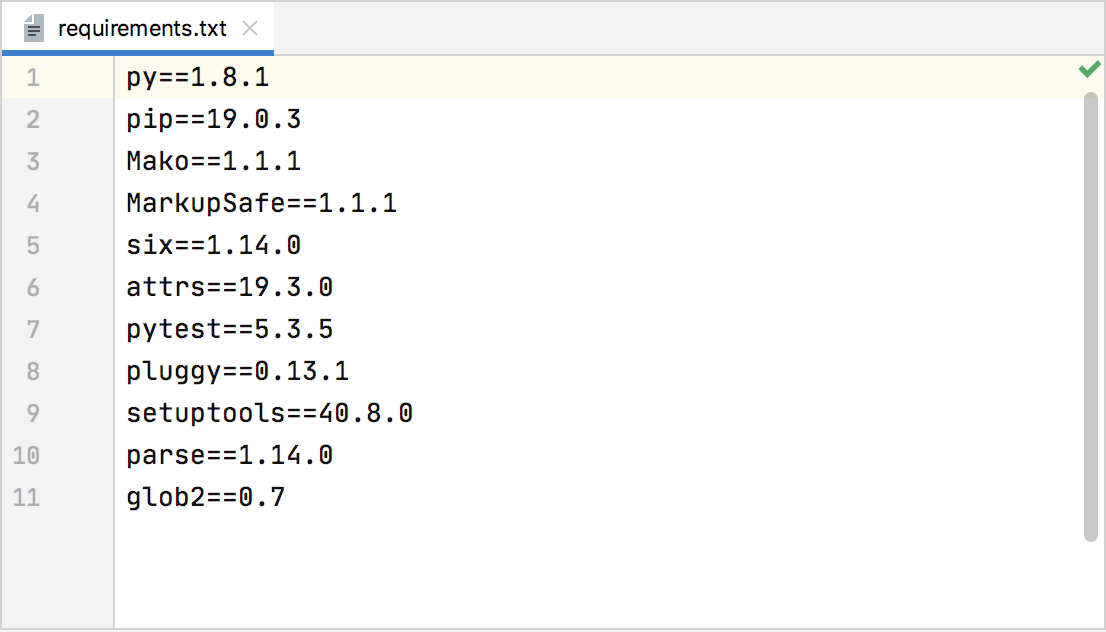
\includegraphics[scale=0.3]{author/part5/figures/pip.png}
	\label{fig:pip}
\end{figure}

Пакетный менеджер \textit{pip} хорошо работает с зависимостями, отображает безуспешно установленные пакеты, а также отображает информацию о требуемой версии пакета при конфликте с другим пакетом.

Альтернативой пакетного менеджера pip является пакетный менеджер \textbf{\textit{poetry}}, который также ориентирован на язык программирования \textit{Python}. Преимущество \textit{poetry} перед \textit{pip} в том, что он автоматически работает с виртуальными окружениями, способен самостоятельно их находить и создавать. Файл конфигурации для пакетов \textit{poetry} является более богатым, чем у pip, он хранит такие сведения, как имя проекта, версия проекта, его описание, лицензия, список авторов, URL проекта, его документации и сайта, список ключевых слов проекта и список \textit{PyPI} классификаторов. \textit{poetry} позволяет более гибко настраивать пакеты для проектов \textit{Python}, файл конфигурации \textit{poetry} представляет собой более богатую спецификацию проекта, однако эта спецификация не позволяет достичь совместимости между компонентами даже в рамках \textit{Python} проектов и предназначена преимущественно только для чтения разработчиком. Автоматизировать проектирование компьютерных систем с помощью пакетного менеджера \textit{poetry} или \textit{pip} невозможно, так как требуется вмешательство разработчика, который должен вручную совместить интерфейсы устанавливаемых пакетов. Другие пакетные менеджеры языков программирования и операционных систем устроены по такому же принципу: существует хранилище компонентов (библиотека), которая представляет собой множество пакетов этого языка программирования или операционной системы и с которым взаимодействует менеджер компонентов.

\begin{figure}[H]
	\caption{Файл конфигурации poetry}
	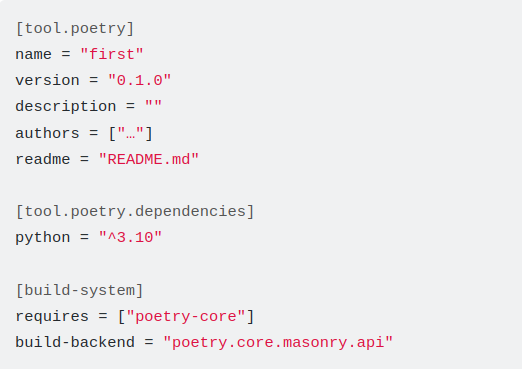
\includegraphics[scale=0.7]{author/part5/figures/poetry.png}
	\label{fig:poetry}
\end{figure}

В качестве компонентного подхода к проектированию программ можно рассмотреть библиотеки подпрограмм современных \textit{языков программирования}, например, \textbf{\textit{Библиотеку STL}} (библиотеку стандартных шаблонов С++).

\textit{Библиотека STL} --- набор согласованных обобщенных алгоритмов, контейнеров, средств доступа к их содержимому и различных вспомогательных функций в C++.

В Библиотеке STL выделяют пять основных компонентов:
\begin{textitemize}
	\item контейнер --- хранение набора объектов в памяти;
	\item итератор --- обеспечение средств доступа к содержимому контейнера;
	\item алгоритм --- определение вычислительной процедуры;
	\item адаптер --- адаптация компонентов для обеспечения различного интерфейса;
	\item функциональный объект --- сокрытие функции в объекте для использования другими компонентами.
\end{textitemize}

\begin{figure}[H]
	\caption{Структура библиотеки STL}
	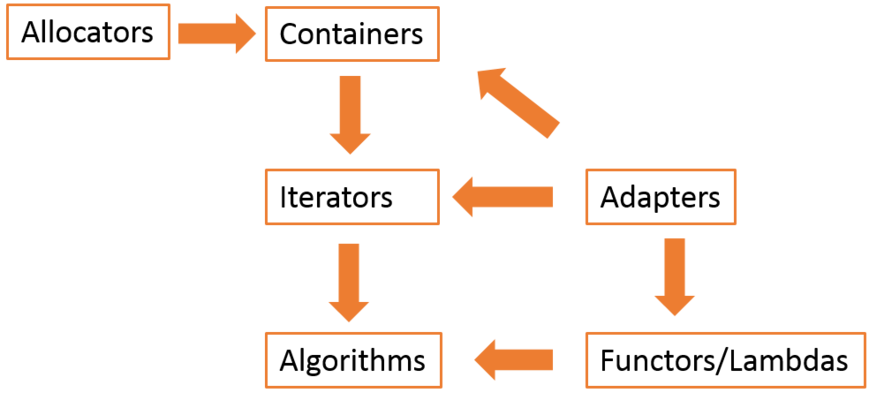
\includegraphics[scale=0.7]{author/part5/figures/STL.png}
	\label{fig:STL}
\end{figure}

Разделение позволяет уменьшить количество компонентов. Например, вместо написания отдельной функции поиска элемента для каждого типа контейнера обеспечивается единственная версия, которая работает с каждым из них, пока соблюдаются основные требования.

Совместимость компонентов (контейнеров) в \textit{Библиотеке STL} обеспечивается общим интерфейсом использования этих компонентов.

Компонентный подход к проектированию компьютерных систем может реализовываться в рамках различных языков, платформ и приложений. Рассмотрим некоторые из них.

Онтология, реализованная на языке \textit{OWL} (Web Ontology Language), представляет собой множество декларативных утверждений о сущностях словаря предметной области (подробнее рассматривается в работе \scncite{Hepp2008}). \textit{OWL} предполагает концепцию "открытого мира"{}, в соответствии с которой применимость описаний предметной области, помещённых в конкретном физическом документе, не ограничивается лишь рамками этого документа --- содержание онтологии может быть использовано и дополнено другими документами, добавляющими новые факты о тех же сущностях или описывающими другую предметную область в терминах данной. "Открытость мира"{} достигается путём добавления URI каждому элементу онтологии, что позволяет воспринимать описанную на \textit{OWL} онтологию как часть всеобщего объединённого знания.

\textbf{\textit{WebProtege}} представляет собой многопользовательский веб-интерфейс, позволяющий редактировать и хранить онтологии в формате \textit{OWL} в совместной среде (см. \scncite{Memduhoglu2018}). Данный проект позволяет не только создавать новые онтологии, но также загружать уже существующие онтологии, которые хранятся на сервере университета Стэнфорда. К преимуществу данного проекта можно отнести автоматическую проверку ошибок в процессе создания объектов онтологий. Данный проект является примером попытки решения проблемы накопления, систематизации и повторного использования уже существующих решений, однако, недостатком данного решения является обособленность разрабатываемых онтологий. Каждый разработанный компонент имеет свою иерархию понятий, подход к выделению классов и сущностей, которые зависят от разработчиков данных онтологий, так как в рамках данного подхода не существует универсальной модели представления знаний, а также формальной спецификации компонентов, представленных в виде онтологий. Следовательно, возникает проблема их семантической несовместимости, что, в свою очередь, приводит к невозможности повторного использования разработанных онтологий при проектировании баз знаний. Данный факт подтверждается наличием на сервере университета Стэнфорда многообразия различных онтологий на одни и те же темы.

На основе языка \textbf{\textit{Modelica}} разработано большое число свободно доступных библиотек компонентов, одной из которых является библиотека Modelica\_StateGraph2, включающая компоненты для моделирования дискретных событий, реактивных и гибридных систем с помощью иерархических диаграмм состояния (см. \scncite{Fritzson2014}). Основным недостатком систем на базе языка \textit{Modelica} является отсутствие совместимости компонентов и достаточной документации, а также узкая направленность разрабатываемых компонентов.

\textbf{\textit{Microsoft Power Apps}} --- это набор приложений, служб и соединителей, а также платформа данных, которая предоставляет среду разработки для эффективного создания пользовательских приложений для бизнеса. Платформа \textit{Microsoft Power Apps} имеет средства для создания библиотеки многократно используемых компонентов графического интерфейса, а также предварительно созданные модели распознавания текста (чтение визитных карточек или чеков) и средство обнаружение объектов, которые можно подключить к разрабатываемому приложению (см. \scncite{Prakash2022}). Библиотека компонентов \textit{Microsoft Power Apps} представляет собой множество создаваемых пользователем компонентов, которые можно использовать в любых приложениях. Преимущество библиотеки в том, что компоненты могут настраивать свойства по умолчанию, которые можно гибко редактировать в любых приложениях, использующих компоненты. Недостаток в том, что отсутствует семантическая совместимость компонентов, спецификация компонентов, не решена проблема существования семантически эквивалентных компонентов, нету иерархии компонентов и средств поиска этих компонентов. Компоненты платформы \textit{Microsoft Power Apps} являются многократно используемыми только для однотипных приложений, которые создаются одним и тем же разработчиком.

\textbf{\textit{Платформа IACPaaS}} (Intelligent Applications, Control and Platform as a Service, см. \scncite{Moskalenko2016}) --- облачная платформа для разработки, управления и удаленного использования интеллектуальных облачных сервисов. Она предназначена для обеспечения поддержки разработки, управления и удаленного использования прикладных и инструментальных мультиагентных облачных сервисов (прежде всего интеллектуальных) и их компонентов для различных предметных областей. Платформа предоставляет доступ:
\begin{textitemize}
	\item прикладным пользователям (специалистам в различных предметных областях) --- к прикладным сервисам;
	\item разработчикам прикладных и инструментальных сервисов и их компонентов --- к инструментальным сервисам;
	\item управляющим интеллектуальными сервисами;
	\item к сервисам управления.
\end{textitemize}

\textit{Платформа IACPaaS} поддерживает:

\begin{textitemize}
	\item базовую технологию разработки прикладных и специализированных инструментальных (интеллектуальных) сервисов с использованием базовых инструментальных сервисов платформы, поддерживающих эту технологию;
	\item множество специализированных технологий разработки прикладных и специализированных инструментальных (интеллектуальных) сервисов, с использованием специализированных инструментальных сервисов платформы, поддерживающих эти технологии.
\end{textitemize}

\textit{Платформа IACPaaS} также не имеет средств для унифицированного представления компонентов интеллектуальных компьютерных систем и средств для их спецификации и автоматической интеграции компонентов.

Исходя из проведённого анализа можно сказать, что на текущем состоянии развития информационных технологий \myuline{не существует} комплексной библиотеки многократно используемых семантически совместимых компонентов компьютерных систем. Таким образом, предлагается комплексная библиотека многократно используемых семантически совместимых компонентов ostis-систем.

\section{Комплексная библиотека многократно используемых семантически совместимых компонентов ostis-систем}
\label{ostis_library_section}

\begin{SCn}
\begin{scnrelfromlist}{ключевой знак}
	\scnitem{Библиотека Метасистемы OSTIS}
	\scnitem{Пример интеграции многократно используемого компонента ostis-систем}
\end{scnrelfromlist}
\end{SCn}

\begin{SCn}
\begin{scnrelfromlist}{ключевое понятие}
	\scnitem{библиотека многократно используемых компонентов ostis-систем}
	\scnitem{материнская ostis-система}
	\scnitem{дочерняя ostis-система}
\end{scnrelfromlist}
\end{SCn}

\begin{SCn}
\begin{scnrelfromlist}{ключевое знание}
	\scnitem{Архитектура Экосистемы OSTIS с точки зрения библиотек многократно используемых компонентов}
	\scnitem{Функциональные возможности библиотеки многократно используемых компонентов ostis-систем}
	\scnitem{Декомпозиция библиотеки многократно используемых компонентов ostis-систем}
\end{scnrelfromlist}
\end{SCn}

\bigskip

Основным требованием, предъявляемым к \textit{Технологии OSTIS}, является обеспечение возможности совместного использования в рамках \textit{ostis-систем} различных \textit{видов знаний} и различных \textit{моделей решения задач} с возможностью \myuline{неограниченного} расширения перечня используемых в \textit{ostis-системе} \textit{видов знаний} и \textit{моделей решения задач} без существенных трудозатрат, а также различных видов интерфейсов. Следствием данного требования является необходимость реализации компонентного подхода на всех уровнях, от простых компонентов баз знаний, решателей задач и интерфейсов до целых \textit{встраиваемых ostis-систем} (понятие компонента рассматривается далее в \textit{\ref{reusable_component_section}}). Интеллектуальная система, спроектированная по \textit{Технологии OSTIS}, представляет собой интеграцию \textit{многократно используемых компонентов баз знаний}, \textit{многократно используемых компонентов решателей задач} и \textit{многократно используемых компонентов интерфейсов} (см. \scncite{Pivovarchik2015}). Различные \textit{многократно используемые компоненты ostis-систем} объединяются в \textit{библиотеки многократно используемых компонентов ostis-систем}. Разработчики \myuline{любой} ostis-системы могут включить в ее состав библиотеку, которая позволит им накапливать и распространять результаты своей деятельности среди других участников \textit{Экосистемы OSTIS} в виде \textit{многократно используемых компонентов}. Решение о включении компонента в библиотеку принимается экспертным сообществом разработчиков, ответственным за качество этой библиотеки. Верификацию компонентов можно автоматизировать путем проверки наличия обязательной части их спецификации, а также тестированием корректности автоматической установки и интеграции компонентов.

В рамках \textit{Экосистемы OSTIS} существует \myuline{множество} библиотек многократно используемых компонентов ostis-систем, являющихся подсистемами соответствующих \textit{материнских ostis-систем}. Все библиотеки в рамках \textit{Экосистемы OSTIS} объединяются в \textit{Библиотеку Экосистемы OSTIS}. Материнская ostis-система отвечает за какой-то класс компонентов и является САПРом для этого класса, содержит методики разработки таких компонентов, их классификацию, подробные пояснения ко всем подклассам компонентов. Таким образом, формируется иерархия \textbf{\textit{материнских ostis-систем}}. \textit{материнская ostis-система} в свою очередь может являться дочерней \textit{ostis-системой} для какой-либо другой \textit{ostis-системы}, заимствуя компоненты из библиотеки, входящей в состав этой другой \textit{ostis-системы}.

\begin{SCn}
	\scnheader{ostis-система}
	\scnsuperset{материнская ostis-система}
	\begin{scnindent}
		\scnidtf{ostis-система, имеющая в своем составе библиотеку многократно используемых компонентов.}
		\scnhaselement{Метасистема OSTIS}
	\end{scnindent}
	\scnsuperset{дочерняя ostis-система}
	\begin{scnindent}
		\scnidtf{ostis-система, в составе которой имеется компонент, заимствованный из какой-либо библиотеки многократно используемых компонентов.}
	\end{scnindent}
\end{SCn}

Библиотека многократно используемых компонентов ostis-систем позволяет использовать проектный опыт по разработке и модернизации ostis-систем различного назначения.

\begin{SCn}
	\scnheader{библиотека многократно используемых компонентов ostis-систем}
	\scntext{часто используемый sc-идентификатор}{библиотека компонентов ostis-систем}
	\scntext{часто используемый sc-идентификатор}{библиотека компонентов}
	\scnidtf{библиотека совместимых многократно используемых компонентов}
	\scnidtf{комплексная библиотека многократно используемых семантически совместимых компонентов ostis-систем}
	\scnidtf{библиотека многократно используемых и совместимых компонентов интеллектуальных компьютерных систем нового поколения}
	\scnidtf{библиотека многократно используемых и совместимых компонентов интеллектуальных компьютерных систем нового поколения}
	\scnidtf{библиотека типовых компонентов ostis-систем}
	\scnidtf{библиотека многократно используемых компонентов OSTIS}
	\scnidtf{библиотека повторно используемых компонентов OSTIS}
	\scnidtf{библиотека intelligent property компонентов ostis-систем}
	\begin{scnindent}
		\scntext{сокращение}{библиотека ip-компонентов ostis-систем}
	\end{scnindent}
	\scnhaselementrole{типичный пример}{\scnkeyword{Библиотека Метасистемы OSTIS}}
	\begin{scnindent}
		\scnidtf{Распределенная библиотека типовых (многократно используемых) компонентов ostis-систем в составе Метасистемы OSTIS}
		\scnidtf{Библиотека многократно используемых компонентов ostis-систем в составе \textit{Метасистемы OSTIS}}
	\end{scnindent}
	\scnhaselementrole{типичный пример}{\scnkeyword{Библиотека Экосистемы OSTIS}}
	\begin{scnindent}
		\scntext{часто используемый sc-идентификатор}{Библиотека OSTIS}
		\scnidtf{Библиотека многократно используемых и совместимых компонентов интеллектуальных компьютерных систем нового поколения}
		\scnidtf{Библиотека типовых компонентов интеллектуальных компьютерных систем нового поколения}
		\scnidtf{Распределенная библиотека типовых (многократно используемых) компонентов ostis-систем в составе Экосистемы OSTIS}
		\scnidtf{Библиотека многократно используемых компонентов ostis-систем в составе \textit{Экосистемы OSTIS}}
	\end{scnindent}
	\begin{scnreltoset}{объединение}
		\scnitem{библиотека многократно используемых компонентов баз знаний ostis-систем (см. \textit{\ref{sc_kb_design_components}~\nameref{sc_kb_design_components})}}
		\scnitem{библиотека многократно используемых компонентов решателей задач ostis-систем (см. \textit{\ref{sec_ps_components}~\nameref{sec_ps_components})}}
		\scnitem{библиотека многократно используемых компонентов интерфейсов ostis-систем (см. \textit{ \ref{sec_reusable_UI_components}~\nameref{sec_reusable_UI_components})}}
		\scnitem{библиотека встраиваемых ostis-систем}
		\scnitem{библиотека ostis-платформ}
	\end{scnreltoset}
\end{SCn}

\myuline{Главной} \textit{библиотекой многократно используемых компонентов ostis-систем} является \textit{Библиотека Метасистемы OSTIS}. \textit{Метасистема OSTIS} (см. \textit{Главу \ref{chapter_ims_standard}~\nameref{chapter_ims_standard}}) выступает \textbf{\textit{материнской системой}} для всех разрабатываемых ostis-систем, поскольку содержит все базовые компоненты (рисунок \textit{\nameref{fig:ecosystem_architecture}}).

\begin{figure}[H]
	\caption{Архитектура Экосистемы OSTIS с точки зрения библиотек многократно используемых компонентов}
	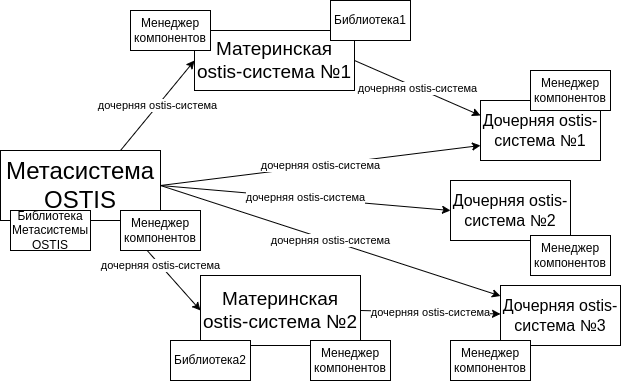
\includegraphics[scale=0.8]{author/part5/figures/ecosystem_architecture.png}
	\label{fig:ecosystem_architecture}
\end{figure}

% Понятие библиотеки Метасистемы OSTIS
Основу для реализации компонентного подхода в рамках \textit{Технологии OSTIS} составляет \textbf{\textit{Библиотека Метасистемы OSTIS}}. \textit{Метасистема OSTIS} ориентирована на разработку и практическое внедрение методов и средств компонентного проектирования семантически совместимых интеллектуальных систем, которая предоставляет возможность быстрого создания интеллектуальных систем различного назначения. В состав \textit{Метасистемы OSTIS} входит \textbf{\textit{Библиотека Метасистемы OSTIS}}. Сферы практического применения технологии компонентного проектирования семантически совместимых интеллектуальных систем ничем не ограничены.

% Зачем нужна Библиотека OSTIS
Основное назначение \textit{Библиотеки Экосистемы OSTIS} --- создание условий для эффективного, осмысленного и массового проектирования ostis-систем и их компонентов путем создания среды для накопления и совместного использования компонентов ostis-систем. Такие условия осуществляются путем неограниченного расширения постоянно эволюционируемых семантически совместимых ostis-систем и их компонентов, входящих в \textit{Экосистему OSTIS}.

Постоянно расширяемая \textit{Библиотека Экосистемы OSTIS} существенно сокращает сроки разработки новых интеллектуальных компьютерных систем. \textit{библиотека многократно используемых компонентов ostis-систем} позволяет избавиться от дублирования семантически эквивалентных информационных компонентов. А также от многообразия форм технической реализации используемых моделей решения задач.

% Что умеет библиотека ostis-систем
Функциональные возможности библиотеки многократно используемых компонентов ostis-систем (см. \scncite{Koronchik2011}):
\begin{SCn}
	\scnheader{библиотека многократно используемых компонентов ostis-систем}
	\begin{scnrelfromset}{функциональные возможности}
		\scnfileitem{Хранение многократно используемых компонентов ostis-систем и их спецификаций. При этом часть компонентов, специфицированных в рамках библиотеки, могут физически храниться в другом месте ввиду особенностей их технической реализации (например, исходные тексты \textit{ostis-платформы} могут физически храниться в каком-либо отдельном репозитории, но специфицированы как компонент будут в соответствующей библиотеке). В этом случае спецификация компонента в рамках библиотеки должна также включать описание (1) того \myuline{где} располагается компонент и (2) сценария его \myuline{автоматической} установки в дочернюю ostis-систему.}
		\scnfileitem{Просмотр имеющихся компонентов и их спецификаций, а также поиск компонентов по фрагментам их спецификации.}
		\scnfileitem{Хранение сведений о статистике использования компонентов. Например, в каких дочерних ostis-системах какие из компонентов библиотеки и какой версии используются (были скачаны). Это необходимо для учета востребованности того или иного компонента, оценки его важности и популярности.}
		\scnfileitem{Систематизация многократно используемых компонентов ostis-систем.}
		\scnfileitem{Обеспечение версионирования многократно используемых компонентов ostis-систем.}
		\scnfileitem{Поиск зависимостей между многократно используемыми компонентами в рамках библиотеки компонентов.}
		\scnfileitem{Обеспечение автоматического обновления компонентов, заимствованных в дочерние ostis-системы. Данная функция может включаться и отключаться по желанию разработчиков дочерней ostis-системы. Одновременное обновление одних и тех же компонентов во всех системах, его использующих, не должно \myuline{ни в каком контексте} приводить к несогласованности между этими системами. Это требование может оказаться довольно сложным, но без него работа \textit{Экосистемы OSTIS} невозможна.}
	\end{scnrelfromset}
\end{SCn}

\textbf{\textit{библиотека многократно используемых компонентов ostis-систем}} является подсистемой ostis-систем, которая имеет свою базу знаний, свой решатель задач и свой интерфейс. Однако не каждая ostis-система обязана иметь библиотеку компонентов.

\begin{SCn}
	\scnheader{библиотека многократно используемых компонентов ostis-систем}
	\begin{scnrelfromset}{обобщенная декомпозиция}
		\scnitem{база знаний библиотеки многократно используемых компонентов ostis-систем}
		\scnitem{решатель задач библиотеки многократно используемых компонентов ostis-систем}
		\scnitem{интерфейс библиотеки многократно используемых компонентов ostis-систем}
		\begin{scnindent}
			\begin{scnrelfromset}{обобщенная декомпозиция}
				\scnitem{минимальный интерфейс библиотеки многократно используемых компонентов ostis-систем}
				\scnitem{расширенный интерфейс библиотеки многократно используемых компонентов ostis-систем}
				\begin{scnindent}
					\scnidtf{графический интерфейс библиотеки многократно используемых компонентов ostis-систем}
					\scnrelfrom{включение}{SCg-интерфейс библиотеки многократно используемых компонентов ostis-систем}
				\end{scnindent}
			\end{scnrelfromset}
		\end{scnindent}
	\end{scnrelfromset}
\end{SCn}

\textbf{\textit{решатель задач библиотеки многократно используемых компонентов ostis-систем}} реализует функциональные возможности библиотеки ostis-систем.

\textbf{\textit{база знаний библиотеки многократно используемых компонентов ostis-систем}} представляет собой иерархию многократно используемых компонентов ostis-систем и их спецификаций.

\textbf{\textit{интерфейс библиотеки многократно используемых компонентов ostis-систем}} обеспечивает доступ к многократно используемым компонентам и возможностям библиотеки ostis-систем для пользователя и других систем (см. \scncite{Koronchik2011}). Существует минимальный и расширенный интерфейс библиотеки многократно используемых компонентов ostis-систем. \textit{минимальный интерфейс библиотеки компонентов} позволяет \textit{менеджеру многократно используемых компонентов ostis-систем}, входящему в состав какой-либо дочерней ostis-системы, подключиться к библиотеке многократно используемых компонентов ostis-систем и использовать ее функциональные возможности, то есть, например, получить доступ к спецификации компонентов и установить выбранные компоненты в \textit{дочернюю ostis-систему}, получить сведения о доступных версиях компонента, его зависимостях и так далее. \textit{расширенный интерфейс библиотеки компонентов}, в отличие от минимального интерфейса, позволяет не только получить доступ к компонентам для дальнейшей работы с ними, но и просматривать существующую структуру библиотеки, а также компоненты и их элементы в удобном и интуитивно понятном для пользователя виде.

% Как происходит интеграция компонентов
Проблема интеграции многократно используемых компонентов ostis-систем решается путём взаимодействия компонентов через общую базу знаний. Компоненты могут лишь использовать общие ключевые узлы (понятия) в базе знаний (см. \scncite{Davydenko2013}, \scncite{Ivashenko2013} и \scncite{Golenkov2014b}). Интеграция многократно используемых компонентов ostis-систем сводится к отождествлению ключевых узлов (см. \textit{\ref{sec_ontological_formalization_basic_denotational_semantics_sc-code}~\nameref{sec_ontological_formalization_basic_denotational_semantics_sc-code}}) и устранению возможных дублирований и противоречий исходя из спецификации компонента и его содержания. Такой способ интеграции компонентов позволяет разрабатывать их параллельно и независимо друг от друга, что значительно сокращает сроки проектирования. Отождествление sc-элементов происходит в ходе выполнения \textit{действие. отождествить два указанных sc-элемента}, которое рассматривается в \textit{Главе \ref{chapter_situation_management}} Автоматическая интеграция компонентов \textit{интеллектуальных систем} представляет широкие возможности для существенного сокращения сроков проектирования \textit{интеллектуальных систем}, поскольку позволяет использовать опыт прошлых разработок.

Рассмотрим пример интеграции многократно используемого компонента \textit{решателей задач}, который представляет собой sc-агент поиска кратчайшего пути в графе, в систему управления логистическими процессами. Допустим, система управления логистическими процессами умеет решать задачи, связанные с оптимизацией издержек в процессе создания товара и со складированием товаров. 

\begin{figure}[H]
	\caption{Структура системы управления логистическими процессами}
	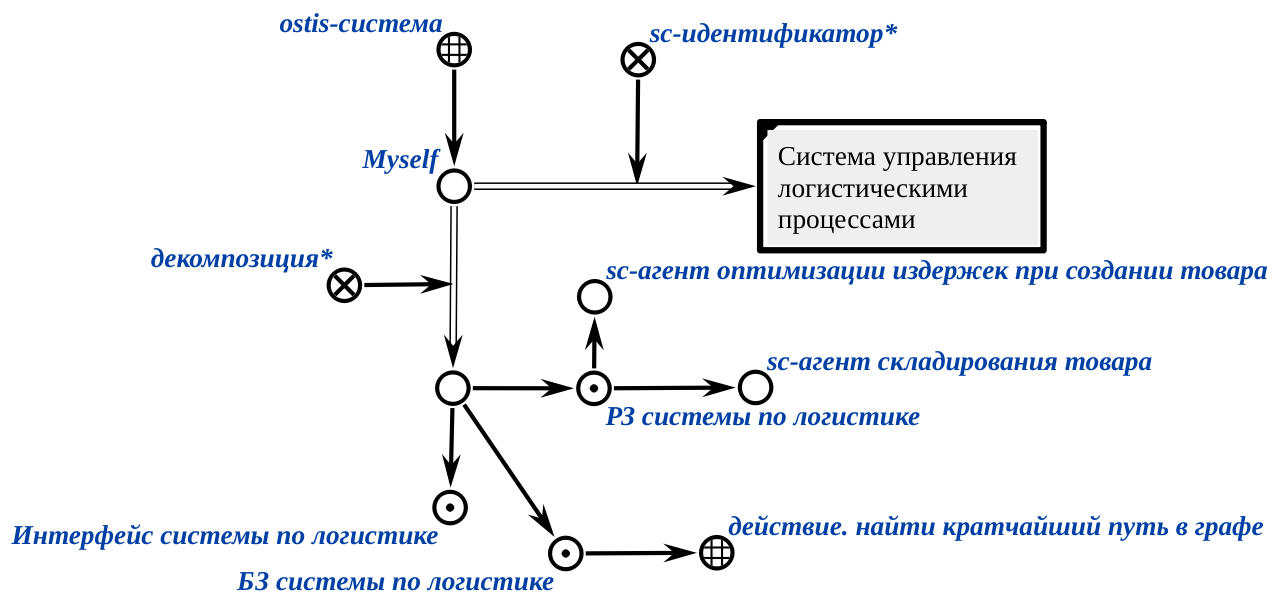
\includegraphics[scale=0.5]{author/part5/figures/logistics_system.png}
	\label{fig:logistics_system}
\end{figure}

При этом в базе знаний системы описано, какие задачи должна решать система и соответствующие им действия. Например, действие. найти кротчайший путь в графе, которое система пока что не умеет выполнять.

Система решения задач по теории графов имеет богатую \textit{базу знаний} и \textit{решатель задач}, в том числе имеет sc-агент поиска кратчайшего пути в графе, который специфицирован как многократно используемый компонент и может быть использован в системе по логистике.

\begin{figure}[H]
	\caption{Структура системы решения задач по теории графов}
	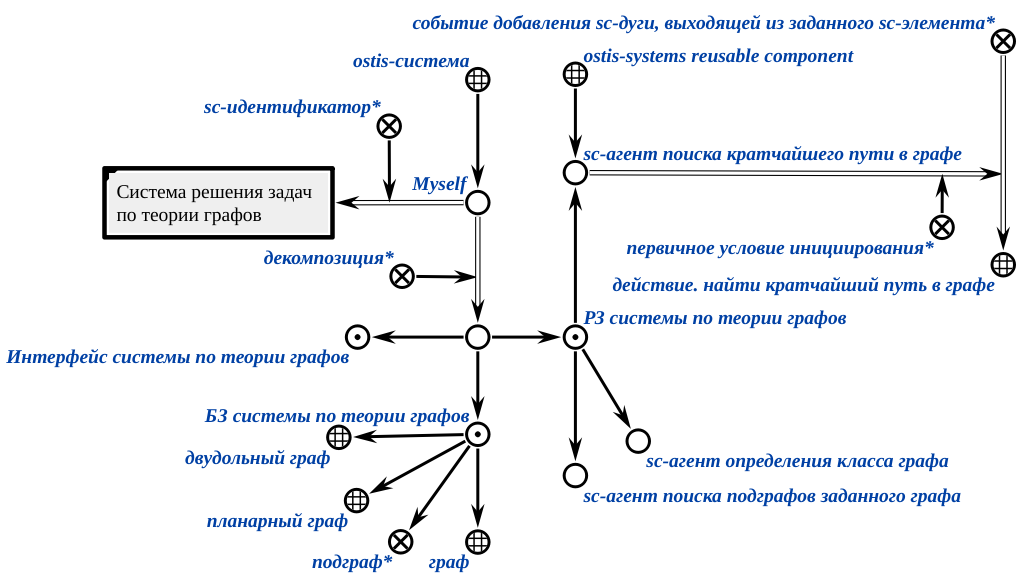
\includegraphics[scale=0.4]{author/part5/figures/graph_theory_system.png}
	\label{fig:graph_theory_system}
\end{figure}

В результате установки \textit{многократно используемого компонента} в виде sc-агента поиска кратчайшего пути в графе вся его sc-модель погружается в систему решения задач по логистике. При интеграции многократно используемого компонента, который представляет собой sc-агент поиска кратчайшего пути в графе, в систему по логистике ключевой узел \textit{действие. найти кратчайший путь в графе} системы по логистике отождествляется с таким же узлом из установленного компонента из системы по теории графов. Таким образом, при выполнении логистических задач, система сможет интерпретировать действие по поиску кратчайших путей с помощью интегрированного компонента.

% Кто еще говорит про интеграцию фрагментов БЗ? В главе Сашеньки не рассматривается. В смысловом пространстве? 
Интеграция любых компонентов ostis-систем происходит автоматически, \myuline{без} вмешательства разработчика. Это достигается за счет использования \textit{SC-кода} и его преимуществ, унификации спецификации многократно используемых компонентов и тщательного отбора компонентов в библиотеках экспертным сообществом, ответственным за эту библиотеку.

\section{Понятие многократно используемого компонента ostis-систем}
\label{reusable_component_section}

\begin{SCn}
\begin{scnrelfromlist}{ключевой знак}
	\scnitem{Пример многократно используемого компонента баз знаний}
	\scnitem{Пример шаблона семантической окрестности отношения}
	\scnitem{Пример обязательной части спецификации многократно используемого компонента ostis-систем}
	\scnitem{Пример необязательной части спецификации многократно используемого компонента ostis-систем}
\end{scnrelfromlist}
\end{SCn}

\begin{SCn}
\begin{scnrelfromlist}{ключевое понятие}
	\scnitem{многократно используемый компонент ostis-систем}
	\scnitem{компонент ostis-системы}
	\scnitem{отношение, специфицирующее многократно используемый компонент ostis-систем}
	\scnitem{встраиваемая ostis-система}
\end{scnrelfromlist}
\end{SCn}

\begin{SCn}
\begin{scnrelfromlist}{ключевое знание}
	\scnitem{Отличие многократно используемого компонента ostis-систем от компонента ostis-системы}
	\scnitem{Требования, предъявляемые к многократно используемым компонентам ostis-систем}
	\scnitem{Классификация многократно используемых компонентов ostis-систем}
	\scnitem{спецификация многократно используемых компонентов ostis-систем}
	\scnitem{Метод установки динамически устанавливаемого многократно используемого компонента ostis-систем}
	\scnitem{Метод установки многократно используемого компонента, при установке которого система требует перезапуска}
\end{scnrelfromlist}
\end{SCn}

\bigskip

Рассмотрим понятие \textbf{\textit{многократно используемого компонента ostis-систем}}. Под многократно используемым компонентом ostis-систем понимается компонент некоторой ostis-системы, который может быть использован в рамках другой ostis-системы (см. \scncite{Shunkevich2015a}). Это компонент ostis-системы, который может быть использован в других ostis-системах (\textbf{\textit{дочерних ostis-системах}}) и содержит все те и только те sc-элементы, которые необходимы для функционирования компонента в дочерней ostis-системе. Другими словами это компонент некоторой \textbf{\textit{материнской ostis-системы}}, который может быть использован в некоторой дочерней ostis-системе. Для включения многократно используемого компонента в некоторую систему, его необходимо установить в эту систему, то есть скопировать в нее все sc-элементы компонента и, при необходимости, вспомогательные файлы, такие как исходные или скомпилированные файлы компонента. \textit{многократно используемые компоненты} должны иметь \myuline{унифицированную} спецификацию и иерархию для поддержки \myuline{совместимости} с другими компонентами. Совместимость многократно используемых компонентов приводит систему к новому качеству, к дополнительному расширению множества решаемых задач при интеграции компонентов.

\begin{SCn}
	\scnheader{многократно используемый компонент ostis-систем}
	\scnidtf{типовой компонент ostis-систем}
	\scnidtf{повторно используемый компонент ostis-систем}
	\scnidtf{многократно используемый компонент OSTIS}
	\scnidtf{ip-компонент ostis-систем}
	\scnidtftext{часто используемый sc-идентификатор}{многократно используемый компонент}
	\scnsubset{компонент ostis-системы}
	\scnsubset{sc-структура}
\end{SCn}

\textbf{\textit{компонент ostis-системы}} --- это целостная часть \textit{ostis-системы}, которая содержит все те (и только те) sc-элементы, которые необходимы для ее функционирования в ostis-системе. \textit{многократно используемый компонент ostis-систем} --- это общий компонент (общая часть) для некоторого множества ostis-систем, который многократно используется, дублируется и входит в состав некоторого множества ostis-систем.
\textbf{\textit{Отличие многократно используемого компонента ostis-систем от компонента ostis-системы}} в том, что многократно используемый компонент имеет \myuline{спецификацию, достаточную для установки} этого компонента в \textit{дочернюю ostis-систему}. Спецификация является частью \textit{базы знаний библиотеки многократно используемых компонентов} соответствующей материнской ostis-системы. Есть техническая возможность встроить \textit{многократно используемый компонент ostis-системы} в \textit{дочернюю ostis-систему}.

\textit{Требования, предъявляемые к многократно используемым компонентам ostis-систем}, наследуют общие требования к проектированию программных компонентов, а также включают следующие:
\begin{textitemize}
	\item существует техническая возможность встроить многократно используемый компонент в дочернюю ostis-систему;
	\item многократно используемый компонент должен выполнять свои функции наиболее общим образом, чтобы круг возможных систем, в которые он может быть встроен, был наиболее широким;
	\item совместимость многократно используемого компонента: компонент должен стремиться повышать уровень \myuline{договороспособности} ostis-систем, в которые он встроен и иметь возможность \myuline{автоматической} интеграции в другие системы;
	\item самодостаточность компонентов (или групп компонентов) технологии, то есть способности их функционировать отдельно от других компонентов без утраты целесообразности их использования.
\end{textitemize}

Рассмотрим \textit{классификацию многократно используемых компонентов ostis-систем} (см. \scncite{Shunkevich2015a} и \scncite{Orlov2022a}). Класс многократно используемого компонента ostis-систем является важной частью спецификации компонента, позволяющей лучше понять назначение и область применения данного компонента, а также класс многократно используемого компонента является важнейшим критерием поиска компонентов в библиотеке ostis-систем. Основной признак классификации многократно используемых компонентов является признак \textit{предметной области}, к которой относится компонент. Здесь структура может быть довольно богатой в соответствии с иерархией областей человеческой деятельности. Существует также множество предметно-независимых многократно используемых компонентов, которые могут использоваться в любой предметной области.

\begin{SCn}
\scnheader{многократно используемый компонент ostis-систем}
\begin{scnrelfromset}{разбиение}
	\scnitem{многократно используемый компонент баз знаний ostis-систем}
	\begin{scnindent}
		\scnidtf{многократно используемый компонент баз знаний}
		\scnsuperset{семантическая окрестность}
		\begin{scnindent}
			\scnhaselement{Семантическая окрестность города Минска}
			\scnhaselement{Семантическая окрестность понятия множество}
		\end{scnindent}
		\scnsuperset{предметная область и онтология}
		\begin{scnindent}
			\scnhaselement{Предметная область и онтология треугольников}
		\end{scnindent}
		\scnsuperset{шаблон многократно используемого компонента ostis-систем}
		\begin{scnindent}
			\scnhaselement{Шаблон описания предметной области}
			\scnhaselement{Шаблон описания отношения}
		\end{scnindent}
	\end{scnindent}
	\scnitem{многократно используемый компонент решателей задач ostis-систем}
	\begin{scnindent}
		\scnidtf{многократно используемый компонент решателей задач}
		\scnsuperset{атомарный абстрактный sc-агент}
		\begin{scnindent}
			\scnhaselement{Абстрактный sc-агент подсчета мощности множества}
		\end{scnindent}
		\scnsuperset{программа обработки знаний}
		\scnsuperset{scp-машина}
		\scnsuperset{scl-машина}
	\end{scnindent}
	\scnitem{многократно используемый компонент интерфейсов ostis-систем}
	\begin{scnindent}
		\scnidtf{многократно используемый компонент интерфейсов}
		\scnsuperset{многократно используемый компонент пользовательских интерфейсов ostis-систем}
	\end{scnindent}
\end{scnrelfromset}
\end{SCn}	

На рисунке \textit{\nameref{fig:set_neighbourhood}} приведен фрагмент \textit{многократно используемого компонента баз знаний} на примере семантической окрестности понятия \textit{множество}.

\begin{figure}[H]
	\caption{Пример многократно используемого компонента баз знаний}
	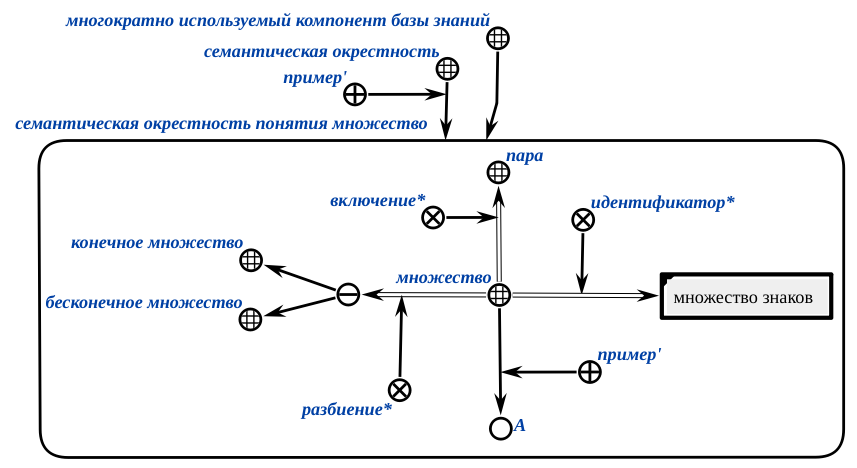
\includegraphics[scale=0.6]{author/part5/figures/set_neighbourhood.png}
	\label{fig:set_neighbourhood}
\end{figure}

На рисунке \textit{\nameref{fig:relation_template}} приведен фрагмент \textit{шаблона многократно используемого компонента ostis-систем} на примере описания семантической окрестности отношения. Шаблоны многократно используемых компонентов также можно использовать для описания платформенно-независимых компонентов решателей задач и интерфейсов.

\begin{figure}[H]
	\caption{Пример шаблона семантической окрестности отношения}
	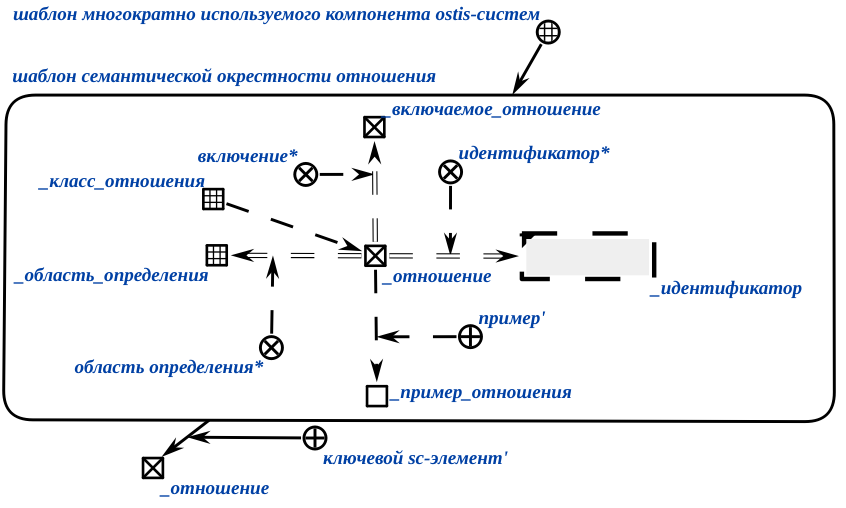
\includegraphics[scale=0.6]{author/part5/figures/relation_template.png}
	\label{fig:relation_template}
\end{figure}

Для компонентов баз знаний важнейшим признаком классификации многократно используемых компонентов является \textit{вид используемых знаний}. Для компонентов решателей задач --- \textit{модель решения задач}. Для компонентов интерфейсов --- \textit{вид интерфейса} в соответствии с классификацией компонентов интерфейсов.

\begin{SCn}
\scnheader{многократно используемый компонент ostis-систем}
\scnrelfrom{разбиение}{\scnkeyword{Типология компонентов ostis-систем по атомарности\scnsupergroupsign}}
\begin{scnindent}
	\begin{scneqtoset}
		\scnitem{атомарный многократно используемый компонент ostis-систем}
		\begin{scnindent}
			\scnhaselement{Абстрактный sc-агент подсчета мощности множества}
		\end{scnindent}
		\scnitem{неатомарный многократно используемый компонент ostis-систем}
		\begin{scnindent}
			\scnidtf{составной многократно используемый компонент ostis-систем}
			\scnhaselement{Решатель задач по геометрии}
		\end{scnindent}
	\end{scneqtoset}
\end{scnindent}
\end{SCn}

\textbf{\textit{атомарный многократно используемый компонент ostis-систем}} --- это \textit{многократно используемый компонент ostis-систем}, который в текущем состоянии библиотеки ostis-систем рассматривается как неделимый, то есть не содержит в своем составе других компонентов. Принадлежность \textit{многократно используемого компонента ostis-систем} классу атомарных компонентов зависит от того, как специфицирован этот компонент и от существующих на данный момент компонентов в библиотеке. \textit{неатомарный многократно используемый компонент} в текущем состоянии библиотеки ostis-систем содержит в своем составе другие атомарные или неатомарные компоненты, он не зависит от своих частей. Без какой-либо части неатомарного компонента его назначение сужается. В общем случае атомарный компонент может перейти в разряд неатомарных в случае, если будет принято решение выделить какую-то из его частей в качестве отдельного компонента. Все вышесказанное, однако, не означает, что даже в случае его платформенной независимости, атомарный компонент всегда хранится в sc-памяти как сформированная sc-структура. Например, платформенно-независимая реализация sc-агента всегда будет представлена набором \textit{scp-программ}, но будет \textit{атомарным многократно используемым компонентом OSTIS} в случае, если ни одна из этих программ не будет представлять интереса как самостоятельный компонент. В общем случае неатомарный компонент может перейти в разряд атомарных в случае, если будет принято решение по каким-либо причинам исключить все его части из рассмотрения в качестве отдельных компонентов. Следует отметить, что неатомарный компонент необязательно должен складываться \myuline{полностью} из других компонентов, в его состав могут также входить и части, не являющиеся самостоятельными компонентами. Например, в состав реализованного на \textit{Языке SCP} \textit{sc-агента}, являющего \textit{неатомарным многократно используемым компонентом} могут входить как \textit{scp-программы}, которые могут являться многократно используемыми компонентами (а могут и не являться), а также агентная \textit{scp-программа}, которая не имеет смысла как многократно используемый компонент.

\begin{SCn}
\scnheader{многократно используемый компонент ostis-систем}
\scnrelfrom{разбиение}{\textbf{\textit{Типология компонентов ostis-систем по зависимости\scnsupergroupsign}}}
\begin{scnindent}
	\begin{scneqtoset}
		\scnitem{зависимый многократно используемый компонент ostis-систем}
		\begin{scnindent}
			\scnhaselement{визуальный редактор системы по химии}
		\end{scnindent}
		\scnitem{независимый многократно используемый компонент ostis-систем}
		\begin{scnindent}
			\scnhaselement{предметная область чисел}
		\end{scnindent}
	\end{scneqtoset}
\end{scnindent}
\end{SCn}

\textbf{\textit{зависимый многократно используемый компонент ostis-систем}} зависит хотя бы от одного другого компонента библиотеки ostis-систем и не может функционировать в дочерней ostis-системе без компонентов, от которых он зависит. \textit{независимый многократно используемый компонент ostis-систем} не зависит ни от одного другого компонента библиотеки ostis-систем.

\begin{SCn}
\scnheader{многократно используемый компонент ostis-систем}
\scnrelfrom{разбиение}{\scnkeyword{Типология компонентов ostis-систем по способу их хранения\scnsupergroupsign}}
\begin{scnindent}
	\begin{scneqtoset}
		\scnitem{многократно используемый компонент ostis-систем, хранящийся в виде внешних файлов}
		\begin{scnindent}
			\begin{scnrelfromset}{разбиение}
				\scnitem{многократно используемый компонент ostis-систем, хранящийся в виде файлов исходных текстов}
				\scnitem{многократно используемый компонент ostis-систем, хранящийся в виде скомпилированных файлов}
			\end{scnrelfromset}
		\end{scnindent}
		\scnitem{многократно используемый компонент, хранящийся в виде sc-структуры}
	\end{scneqtoset}
\end{scnindent}
\end{SCn}

На данном этапе развития \textit{Технологии OSTIS} более удобным является хранение компонентов в виде исходных текстов.

\begin{SCn}
\scnheader{многократно используемый компонент ostis-систем}
\scnrelfrom{разбиение}{\scnkeyword{Типология компонентов ostis-систем по зависимости от ostis-платформы\scnsupergroupsign}}
\begin{scnindent}
	\begin{scneqtoset}
		\scnitem{платформенно-зависимый многократно используемый компонент ostis-систем}
		\begin{scnindent}
			\scnsuperset{ostis-платформа}
			\scnsuperset{абстрактный sc-агент, не реализуемый на Языке SCP}
		\end{scnindent}
		\scnitem{платформенно-независимый многократно используемый компонент ostis-систем}
		\begin{scnindent}
			\scnsuperset{многократно используемый компонент баз знаний}
			\scnsuperset{платформенно-независимый абстрактный sc-агент}
			\scnsuperset{scp-программа}
		\end{scnindent}
	\end{scneqtoset}
\end{scnindent}
\end{SCn}

Под \textbf{\textit{платформенно-зависимым многократно используемым компонентом ostis-систем}} понимается компонент, частично или полностью реализованный при помощи каких-либо сторонних с точки зрения \textit{Технологии OSTIS} средств. Недостаток таких компонентов в том, что интеграция таких компонентов в интеллектуальные системы может сопровождаться дополнительными трудностями, зависящими от конкретных средств реализации компонента. В качестве возможного преимущества платформенно-зависимых многократно используемых компонентов ostis-систем можно выделить их, как правило, более высокую производительность за счет реализации их на более приближенном к платформе уровне. В общем случае платформенно-зависимый многократно используемый компонент ostis-систем может поставляться как в виде набора исходных кодов, так и в скомпилированном виде. Процесс интеграции платформенно-зависимого многократно используемого компонента ostis-систем в дочернюю систему, разработанную по \textit{Технологии OSTIS}, сильно зависит от технологий реализации данного компонента и в каждом конкретном случае может состоять из различных этапов. Каждый платформенно-зависимый многократно используемый компонент ostis-систем должен иметь соответствующую подробную, корректную и понятную инструкцию по его установке и внедрению в дочернюю систему.

Под \textbf{\textit{платформенно-независимым многократно используемым компонентом ostis-систем}} понимается компонент, который целиком и полностью представлен на \textit{SC-коде}. В случае \textit{неатомарного многократно используемого компонента} это означает, что \myuline{все} более простые компоненты, входящие в его состав также обязаны быть платформенно-независимыми многократно используемыми компонентами ostis-систем. Процесс интеграции платформенно-зависимого многократно используемого компонента ostis-систем в дочернюю систему, разработанную по Технологии OSTIS, существенно упрощается за счет использования общей унифицированной формальной основы представления и обработки знаний.

Наиболее ценными являются \textit{платформенно-независимые многократно используемые компоненты ostis-систем}.

\begin{SCn}
\scnheader{многократно используемый компонент ostis-систем}
\scnrelfrom{разбиение}{\scnkeyword{Типология компонентов ostis-систем по динамичности их установки\scnsupergroupsign}}
\begin{scnindent}
	\begin{scneqtoset}
		\scnitem{динамически устанавливаемый многократно используемый компонент ostis-систем}
		\begin{scnindent}
			\scnidtf{многократно используемый компонент, при установке которого система не требует перезапуска}
			\begin{scnrelfromset}{декомпозиция}
				\scnitem{многократно используемый компонент, хранящийся в виде скомпилированных файлов}
				\scnitem{многократно используемый компонент баз знаний}
			\end{scnrelfromset}
		\end{scnindent}
		\scnitem{многократно используемый компонент, при установке которого система требует перезапуска}
	\end{scneqtoset}
\end{scnindent}
\end{SCn}

Процесс интеграции компонентов разных видов на разных этапах жизненного цикла \textit{osits-систем} бывает разным. Наиболее ценными являются компоненты, которые могут быть интегрированы в работающую систему \myuline{без} прекращения ее функционирования. Некоторые системы, особенно системы управления, нельзя останавливать, а устанавливать и обновлять компоненты нужно.

\textbf{\textit{встраиваемая ostis-система}} --- это \textit{неатомарный многократно используемый компонент}, который состоит из \textit{базы знаний}, \textit{решателя задач} и \textit{интерфейса}.

\begin{SCn}
	\scnheader{встраиваемая ostis-система}
	\scnsubset{ostis-система}
	\scnsubset{неатомарный многократно используемый компонент ostis-систем}
	\begin{scnrelfromset}{декомпозиция}
		\scnitem{многократно используемый компонент баз знаний ostis-систем}
		\scnitem{многократно используемый компонент решателей задач ostis-систем}
		\scnitem{многократно используемый компонент интерфейсов ostis-систем}
	\end{scnrelfromset}
\end{SCn}

Такими системами могут быть, например, интеллектуальный интерфейс (в том числе естественно-языковой интерфейс), \textit{средство коллективного проектирования баз знаний}, \textit{менеджер многократно используемых компонентов ostis-систем}, \textit{интеллектуальная обучающая система}, \textit{система тестирования и верификации интеллектуальных систем}, \textit{визуальный web-ориентированный редактор sc.g-текстов} и другие.

Особенность \textit{встраиваемых ostis-систем} в том, что интеграция целых интеллектуальных систем предполагает интеграцию баз знаний этих систем, интеграцию их решателей задач и интеграцию их интеллектуальных интерфейсов. При интеграции встраиваемых ostis-систем база знаний встраиваемой системы становится частью базы знаний системы, в которую она встраивается. Решатель задач встраиваемой ostis-системы становится частью решателя задач системы, в которую она встраивается. И интерфейс встраиваемой ostis-системы становится частью интерфейса системы, в которую она встраивается. При этом встраиваемая система является целостной и может функционировать отдельно от других ostis-систем, в отличие от других многократно используемых компонентов.

\textit{встраиваемые ostis-системы} зачастую являются предметно-независимыми многократно используемыми компонентами. Таким образом, например, встраиваемая ostis-система в виде среды проектирования баз знаний может быть встроена как в систему из предметной области по геометрии, так и в систему управления аграрными объектами.

\textit{встраиваемая ostis-система}, как и любой другой многократно используемый компонент ostis-систем, должна поддерживать семантическую совместимость ostis-систем. Как сама встраиваемая ostis-система, так и все ее компоненты должны быть специфицированы и согласованы. Компоненты встраиваемых ostis-систем могут быть заменены на другие, имеющие то же назначение, например, естественно-языковой интерфейс может иметь различные варианты базы знаний в зависимости от естественного языка, поддерживаемого системой, различные варианты интерфейса, в зависимости от требований и удобства пользователей и также различные варианты реализации решателя задач для обработки естественного языка, которые могут использовать различные модели, однако решать одну и ту же задачу. Встраиваемая ostis-система связывается с системой, в которую она встроена с помощью отношения \textbf{\textit{встроенная ostis-система*}}, которое является подмножеством отношения \textit{встроенная кибернетическая система*}.

Для того, чтобы хранить \textit{многократно используемые компоненты ostis-систем}, необходимо некоторое хранилище. Таким хранилищем может выступать как какая-либо ostis-система, так и стороннее хранилище, например, облачное. Помимо внешних файлов компонента в хранилище должна находиться его \myuline{спецификация}.

Каждый \textit{многократно используемый компонент ostis-систем} должен быть специфицирован в рамках библиотеки (см. \scncite{Davydenko2013}). Данные спецификации включают в себя основные знания о компоненте, которые позволяют обеспечить построение полной иерархии компонентов и их зависимостей, а также обеспечивают \myuline{беспрепятственную} интеграцию компонентов в дочерние ostis-системы (см. \scncite{Orlov2022a}). Для спецификации компонента используются, как отношения, так и классы компонента.

% Параметры формализовать
Чтобы многократно используемый компонент мог быть принят в библиотеку, нужно специфицировать его, используя отношения класса \textit{необходимое для установки отношение, специфицирующее многократно используемый компонент ostis-систем}. Здесь описана спецификация, общая для любых типов компонентов, однако в зависимости от типа компонента, спецификация может расширяться (см. \textit{\ref{sc_kb_design_components}~\nameref{sc_kb_design_components}, \ref{sec_ps_components}~\nameref{sec_ps_components}, \ref{sec_reusable_UI_components}~\nameref{sec_reusable_UI_components}}). Отношения класса \textit{необязательное для установки отношение, специфицирующее многократно используемый компонент ostis-систем} помогают лучше понять суть компонента, упрощают поиск, но не являются обязательными для того, чтобы компонент мог быть установлен в ostis-систему. Спецификация многократно используемого компонента ostis-систем также включает класс (тип) компонента. Указание класса \textit{многократно используемый компонент ostis-систем} является обязательным. Сам многократно используемый компонент в рамках спецификации является \textit{ключевым sc-элементом}, а также может иметь множество своих ключевых sc-элементов. Для уточнения типа компонента могут использоваться другие классы, например дата публикации первой и последней версии компонента, качественно-количественные характеристики, такие как уровень семантической совместимости компонентов, сложность реализации компонента, уровень производительности компонента (для программ можно использовать O-нотацию), количество sc-элементов, входящих в состав многократно используемого компонента, количество ключевых узлов компонента, рейтинг компонента в рамках \textit{Экосистемы OSTIS}, количество скачиваний компонента и другие (см. \scncite{Davydenko2013}). Параметр \textit{лицензия многократно используемого компонента} используется для обозначения условий использования и распространения компонента. По умолчанию лицензия компонента открытая, если не указано иное.

\begin{SCn}
\scnheader{отношение, специфицирующее многократно используемый компонент ostis-систем}
\scnidtf{отношение, которое используется при спецификации многократно используемого компонента ostis-систем}
\begin{scnrelfromset}{разбиение}
	\scnitem{необходимое для установки отношение, специфицирующее многократно используемый компонент ostis-систем}
	\begin{scnindent}
		\scnhaselement{метод установки*}
		\scnhaselement{адрес хранилища*}
		\scnhaselement{зависимости компонента*}
	\end{scnindent}
	\scnitem{необязательное для установки отношение, специфицирующее многократно используемый компонент ostis-систем}
	\begin{scnindent}
		\scnhaselement{сопутствующие компоненты*}
		\scnhaselement{история изменений*}
		\scnhaselement{модификации компонентов*}
		\scnhaselement{авторы*}
		\scnhaselement{примечание*}
		\scnhaselement{пояснение*}
		\scnhaselement{идентификатор*}
		\scnhaselement{ключевой sc-элемент*}
		\scnhaselement{назначение*}
		\scnhaselement{требования полноты*}
		\scnhaselement{требования безошибочности*}
		\scnhaselement{преимущества*}
		\scnhaselement{недостатки*}
	\end{scnindent}
\end{scnrelfromset}
\end{SCn}

На рисунке \textit{\nameref{fig:component_required_specification_example}} изображена обязательная часть спецификации, необходимой для установки sc-агента поиска кратчайшего пути в графе.

\begin{figure}[H]
	\caption{Пример обязательной части спецификации многократно используемого компонента ostis-систем}
	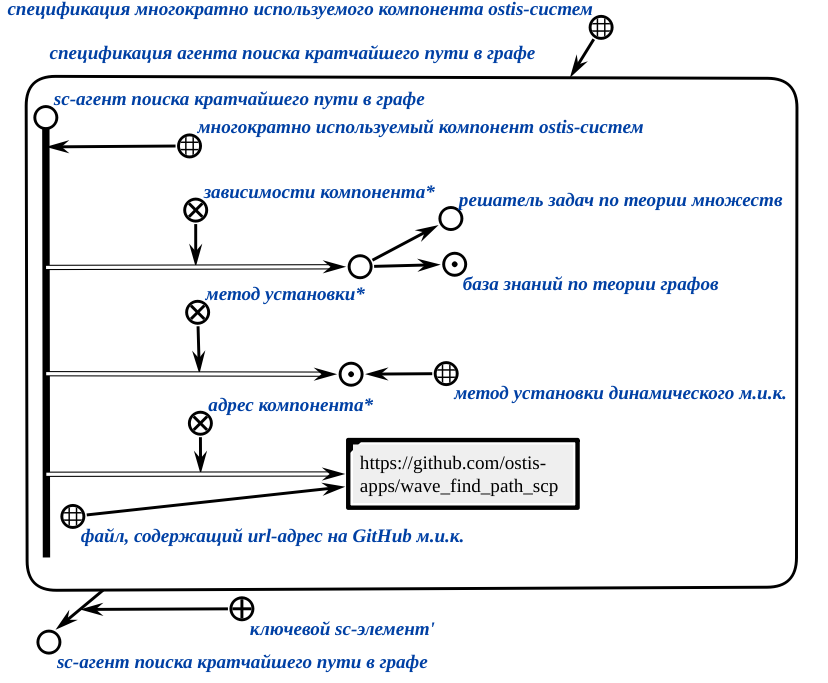
\includegraphics[scale=0.6]{author/part5/figures/component_required_specification_example.png}
	\label{fig:component_required_specification_example}
\end{figure}

Метод установки позволяет пользователю установить компонент вручную, а \textbf{\textit{менеджеру многократно используемых компонентов ostis-систем}} --- автоматически. Основные два метода установки многократно используемых компонентов --- метод установки \myuline{динамически} устанавливаемого многократно используемого компонента ostis-систем и метод установки многократно используемого компонента, при установке которого система \myuline{требует перезапуска}. При динамической установке необходимо только скачать компонент и, при необходимости, его зависимые компоненты, и он сразу же функционирует в системе. 

\begin{figure}[H]
	\caption{Метод установки динамически устанавливаемого многократно используемого компонента ostis-систем}
	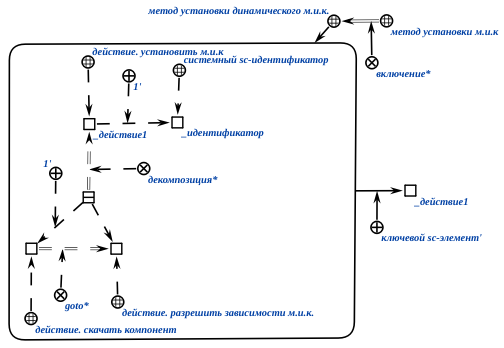
\includegraphics[scale=0.6]{author/part5/figures/install_dynamic_method.png}
	\label{fig:dynamic_method}
\end{figure}

При установке компонента, при установке которого система требует перезапуска, необходимо помимо скачивания компонента транслировать его в память системы.

\begin{figure}[H]
	\caption{Метод установки многократно используемого компонента, при установке которого система требует перезапуска}
	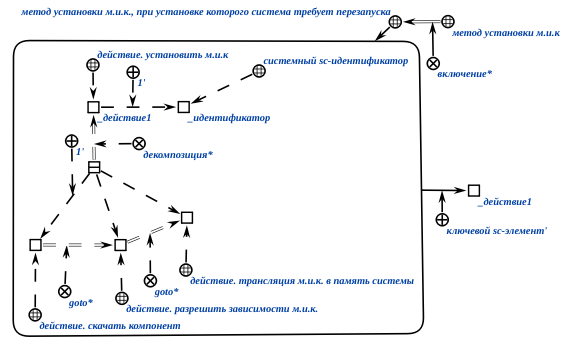
\includegraphics[scale=0.6]{author/part5/figures/install_with_reboot_method.png}
	\label{fig:install_with_reboot_method}
\end{figure}


Связки отношения \textit{адрес хранилища*} связывают многократно используемый компонент, хранящийся в виде внешних файлов и файл, содержащий url-адрес \textit{многократно используемого компонента ostis-систем}. Таким файлом может быть файл, содержащий url-адрес на GitHub \textit{многократно используемого компонента ostis-систем}, файл, содержащий url-адрес на Google Drive многократно используемого компонента ostis-систем, файл, содержащий url-адрес на Docker Hub многократно используемого компонента ostis-систем, и другие.

Связки отношения \textit{зависимости компонента*} связывают многократно используемый компонент и множество компонентов, без которых устанавливаемый компонент \myuline{не может быть} встроен в дочернюю ostis-систему.

Спецификация неатомарного многократно используемого компонента должна содержать информацию о том, из каких компонентов он состоит, используя отношение \textit{декомпозиция*}. При этом sc-структура, обозначающая неатомарный компонент не обязана содержать все sc-элементы компонентов, на которые она декомпозируется, достаточно, чтобы неатомарному компоненту принадлежали знаки всех тех компонентов, из которых он состоит (должно быть полное перечисление составных компонентов).

На рисунке \textit{\nameref{fig:component_optional_specification_example}} изображена необязательная часть спецификации, необходимой для установки sc-агента поиска кратчайшего пути в графе. Полная спецификация компонента является результатом объединения обязательной и необязательной частей. Другие примеры спецификаций многократно используемых компонентов ostis-систем описаны в \textit{\ref{gis_components}~\nameref{gis_components}}.

\begin{figure}[H]
	\caption{Пример необязательной части спецификации многократно используемого компонента ostis-систем}
	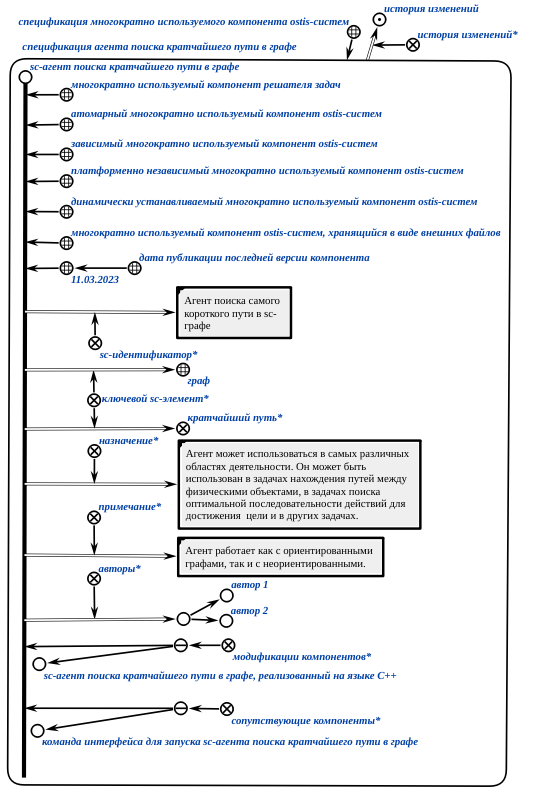
\includegraphics[scale=1.0]{author/part5/figures/component_optional_specification_example.png}
	\label{fig:component_optional_specification_example}
\end{figure}

В некоторых случаях может оказаться, что для использования одного многократно используемого компонента OSTIS целесообразно или даже необходимо дополнительно использовать несколько других \textit{многократно используемых компонентов OSTIS}. Например, может оказаться целесообразным вместе с каким либо sc-агентом информационного поиска использовать соответствующую команду интерфейса, которая представлена отдельным компонентом и позволит пользователю задавать вопрос для указанного sc-агента через интерфейс системы. В таких случаях для связи компонентов используется отношение \textit{сопутствующие компоненты*}. Наличие таких связей позволяет устранить возможные проблемы неполноты знаний и навыков в дочерней системе, из-за которых какие-либо из компонентов могут не выполнять свои функции. Связки отношения \textit{сопутствующий компонент*} связывают многократно используемые компоненты ostis-систем, которые целесообразно использовать в дочерней системе вместе. Каждая такая связка может дополнительно быть снабжена sc-комментарием или sc-пояснением, отражающим суть указываемой зависимости. Отношение \textit{история изменений*} позволяет специфицировать различные версии компонента и, при необходимости, устанавливать выбранную пользователем версию. Различные версии, как правило, отражают какие-либо улучшения или исправления ошибок. \textit{модификации компонентов*} --- это функционально эквивалентные реализации одного и того же компонента, которые могут быть синтаксически эквивалентны (например, реализация одного и того же sc-агента на платформенно-зависимом и платформенно-независимом уровнях). Развитие \textit{Библиотеки Экосистемы OSTIS} происходит не только за счет ее пополнения новыми компонентами, но и за счет появления новых версий и модификаций уже существующих компонентов. Связки отношения \textit{авторы*} связывают многократно используемый компонент со множеством авторов этого компонента. Спецификация может также содержать дополнительную информацию об авторах при необходимости. Отношения \textit{примечание*} и \textit{пояснение*} связывают многократно используемый компонент и некоторый текст (как естественно-языковой, так и текст на SC-коде), который является примечанием или пояснением к этому компоненту. Идентификаторы компонента позволяют пользователям и разработчикам обозначать компонент, используя внешний язык. Ключевые sc-элементы компонента позволяют указать на наиболее важные понятия, связанные с описываемым компонентом. Отношение \textit{назначение*} позволяет описать ожидаемый сценарий, выделить рекомендации использования многократно используемого компонента. Требования полноты и безошибочности специфицируют возможные ограничения и ошибки компонента, область его использования.

\section{Менеджер многократно используемых компонентов ostis-систем}
\label{ostis_library_component_manager}

\begin{SCn}
\begin{scnrelfromlist}{ключевой знак}
	\scnitem{Реализация менеджера многократно используемых компонентов ostis-систем}
	\scnitem{Пример структуры хранилища адресов спецификаций компонентов}
\end{scnrelfromlist}
\end{SCn}

\begin{SCn}
\begin{scnrelfromlist}{ключевое понятие}
	\scnitem{менеджер многократно используемых компонентов ostis-систем}
\end{scnrelfromlist}
\end{SCn}

\bigskip

\begin{SCn}
\begin{scnrelfromlist}{ключевое знание}
	\scnitem{Минимальные функциональные возможности менеджера компонентов}
	\scnitem{Расширенные функциональные возможности менеджера компонентов}
\end{scnrelfromlist}
\end{SCn}

\bigskip

\textbf{\textit{менеджер многократно используемых компонентов ostis-систем}} --- подсистема ostis-системы, с помощью которой происходит взаимодействие с библиотекой компонентов ostis-систем.

\begin{SCn}
\scnheader{менеджер многократно используемых компонентов ostis-систем}
\scnsubset{встраиваемая ostis-система}
\scnsubset{платформенно-зависимый многократно используемый компонент ostis-систем}
\scnidtftext{часто используемый sc-идентификатор}{менеджер многократно используемых компонентов}
\scnidtftext{часто используемый sc-идентификатор}{менеджер компонентов}
\begin{scnrelfromset}{обобщенная декомпозиция}
	\scnitem{база знаний менеджера многократно используемых компонентов ostis-систем}
	\scnitem{решатель задач менеджера многократно используемых компонентов ostis-систем}
	\scnitem{интерфейс менеджера многократно используемых компонентов ostis-систем}
\end{scnrelfromset}
\scnhaselement{Реализация менеджера многократно используемых компонентов ostis-систем}
\begin{scnindent}
	\scntext{адрес компонента}{https://github.com/ostis-ai/sc-component-manager}
\end{scnindent}
\end{SCn}

\textbf{\textit{база знаний менеджера многократно используемых компонентов ostis-систем}} содержит все те знания, которые необходимы для установки многократно используемого компонента в дочернюю ostis-систему. К таким знаниям относятся знания о спецификации многократно используемых компонентов, методы установки компонентов, знание о библиотеках ostis-систем, с которыми происходит взаимодействие, \textit{Классификация компонентов} и другие. \textbf{\textit{решатель задач менеджера многократно используемых компонентов ostis-систем}} взаимодействует с \textit{библиотекой ostis-систем} и позволяет установить и интегрировать многократно используемые компоненты в дочернюю ostis-систему, также выполнять поиск, обновление, публикацию, удаление компонентов и другие операции с ними. \textbf{\textit{интерфейс менеджера многократно используемых компонентов ostis-систем}} обеспечивает удобное для пользователя и других систем использование менеджера компонентов.

\textit{решатель задач менеджера многократно используемых компонентов ostis-систем} как минимум должен обеспечивать следующие функциональные возможности:

\begin{SCn}
\scnheader{менеджер многократно используемых компонентов ostis-систем}
\scnrelfrom{минимальные функциональные возможности}{Минимальные функциональные возможности менеджера компонентов}
\begin{scnindent}
\begin{scneqtoset}
	\scnfileitem{\textbf{Поиск многократно используемых компонентов ostis-систем.} Множество возможных критериев поиска соответствует спецификации многократно используемых компонентов. Такими критериями могут быть классы компонента, его авторы, идентификатор, фрагмент примечания, назначение, принадлежность какой-либо предметной области, вид знаний компонента и другие.}
	\scnfileitem{\textbf{Установка многократно используемого компонента ostis-систем.} Установка многократно используемого компонента происходит вне зависимости от типологии, способа установки и местоположения компонента. Необходимое условие для возможности установки многократно используемого компонента --- наличие \textbf{\textit{спецификации многократно используемого компонента ostis-систем}}. Перед установкой многократно используемого компонента в дочернюю систему необходимо установить все зависимые компоненты. Также для платформенно-зависимых компонентов может быть необходимо установить иные зависимости, которые не являются компонентами какой-либо библиотеки ostis-систем. После успешной установки компонента в базе знаний дочерней системы генерируется информационная конструкция, обозначающая факт установки компонента в систему с помощью отношения \textit{установленные компоненты*}.}
	\scnfileitem{\textbf{Добавление и удаление отслеживаемых менеджером компонентов библиотек.} Менеджер компонентов содержит информацию о множестве источников для установки компонентов, перечень которых можно дополнять. По умолчанию менеджер компонентов отслеживает \textit{Библиотеку Метасистемы OSTIS}, однако можно создавать и добавлять дополнительные библиотеки ostis-систем.}
\end{scneqtoset}
\end{scnindent}
\end{SCn}

Исходя из указанных минимальных функциональных возможностей \textit{решатель задач менеджера многократно используемых компонентов ostis-систем} представляет собой следующую иерархию абстрактных sc-агентов:

\begin{SCn}
	\scnheader{решатель задач менеджера многократно используемых компонентов ostis-систем}
	\begin{scnrelfromset}{декомпозиция абстрактного sc-агента}
		\scnitem{Абстрактный sc-агент поиска многократно используемых компонентов ostis-систем}
		\scnitem{Абстрактный sc-агент установки многократно используемых компонентов ostis-систем}
		\scnitem{Абстрактный sc-агент управления отслеживаемых менеджером компонентов библиотек}
		\begin{scnindent}
			\begin{scnrelfromset}{декомпозиция абстрактного sc-агента}
				\scnitem{Абстрактный sc-агент добавления отслеживаемой менеджером компонентов библиотеки}
				\scnitem{Абстрактный sc-агент удаления отслеживаемой менеджером компонентов библиотеки}
			\end{scnrelfromset}
		\end{scnindent}
	\end{scnrelfromset}
\end{SCn}

Используя минимальные функциональные возможности менеджер компонентов может установить компоненты, которые будут расширять его же функционал. Компоненты, реализующие расширенный функционал менеджера компонентов являются частью \textit{Библиотеки Метасистемы OSTIS}. К расширенному функционалу относится:

\begin{SCn}
\scnheader{менеджер многократно используемых компонентов ostis-систем}
\scnrelfrom{расширенные функциональные возможности}{Расширенные функциональные возможности менеджера компонентов}
\begin{scnindent}
	\begin{scneqtoset}
		\scnfileitem{\textbf{Спецификация} многократно используемого компонента ostis-систем. Менеджер компонентов позволяет специфицировать компоненты, входящие в состав библиотеки ostis-систем, а также специфицировать новые создаваемые компоненты, которые будут публиковаться в библиотеку ostis-систем. При этом спецификация может происходить как автоматически, так и вручную. Например, менеджер компонентов может обновить спецификацию используемого компонента в соответствии с тем, в какие новые ostis-системы его установили, обновить спецификацию авторства компонента при его редактировании в библиотеке ostis-систем, спецификацию ошибок, выявленных в процессе эксплуатации компонента и так далее.}
		\scnfileitem{\textbf{Формирование} многократно используемого компонента ostis-систем по шаблону с заданными параметрами. При установке шаблона многократно используемого компонента ostis-систем менеджер компонентов позволяет сформировать по нему конкретный компонент. Для этого пользователю предлагается определить значения всех sc-переменных в шаблоне для формирования конкретного компонента из некоторой предметной области. Например, для формирования многократно используемого компонента баз знаний, представляющего собой семантическую окрестность некоторого отношения (см. рисунок \textit{\nameref{fig:relation_template}}), нужно определить значения всех переменных, кроме переменной, являющейся ключевым sc-элементом данной структуры.}
		\scnfileitem{\textbf{Публикация} многократно используемого компонента ostis-систем в библиотеку ostis-систем. При публикации компонента в библиотеку ostis-систем происходит верификация на основе спецификации компонента. Публикация компонента может сопровождаться сборкой неатомарного компонента из существующих атомарных. Также существует возможность обновления версии опубликованного компонента сообществом его разработчиков.}
		\scnfileitem{\textbf{Обновление} установленного многократно используемого компонента ostis-систем.}
		\scnfileitem{\textbf{Удаление} установленного многократно используемого компонента. Как и в случае установки после удаления многократно используемого компонента из ostis-системы в базе знаний системы устанавливается факт удаления компонента. Эта информация является важной частью \myuline{истории эксплуатации} ostis-системы.}
		\scnfileitem{\textbf{Редактирование} многократно используемого компонента в библиотеке ostis-систем.}
		\scnfileitem{\textbf{Сравнение} многократно используемых компонентов ostis-систем.}
	\end{scneqtoset}
\end{scnindent}
\end{SCn}

Для того, чтобы создать новую ostis-систему "с нуля"{}, используя \textit{ostis-платформу} (см. \textit{\ref{sec_interpreter_ostis_platform}~\nameref{sec_interpreter_ostis_platform}}), необходимо установить некоторый \textit{Программный вариант реализации ostis-платформы} (см. Главу \textit{\ref{chapter_soft_platform}~\nameref{chapter_soft_platform}}) с помощью сторонних средств. Такими средствами могут быть (1) хранилища исходного кода платформы, например, облачные хранилища, такие как GitHub репозиторий, с соответствующим набором инструкций по установке платформы или (2) средства установки заранее скомпилированной программной реализации платформы, например, средство установки программного обеспечения apt. Далее установка многократно используемых компонентов в ostis-систему (независимо от типа компонентов) осуществляется с помощью менеджера компонентов. При установке платформенно-зависимых компонентов менеджер компонентов должен управлять соответствующими средствами сборки таких компонентов (CMake, Ninja, npm, grunt и другие).

Компонент находится в некотором хранилище --- (1) \textit{библиотеке компонентов ostis-систем} или (2) в виде файлов в некотором облачном хранилище. В случае, когда компонент хранится в библиотеке, для его установки менеджер компонентов копирует все sc-элементы, которые представляют собой компонент, в дочернюю ostis-систему. В случае, когда компонент хранится в виде файлов в облачном хранилище, менеджер компонентов скачивает файлы компонента и устанавливает их в соответствии со спецификацией. Адреса хранилищ спецификаций компонентов должны храниться в базе знаний менеджера компонентов, чтобы иметь доступ к спецификациям компонентов для их последующего использования (поиска, установки и так далее). На рисунке \textit{\nameref{fig:specification_storage_addresses}} приведен пример фрагмента базы знаний менеджера компонентов, который описывает то, где хранятся спецификации компонентов, доступных для установки. Такое хранилище представляет собой множество, состоящее из двух множеств: (1) множество адресов спецификаций компонентов и (2) множество адресов спецификаций других хранилищ. Таким образом, образуется древовидная структура в соответствии с иерархией материнских ostis-систем и соответствующих им библиотек.

\begin{figure}[H]
	\caption{Пример структуры хранилища адресов спецификаций компонентов}
	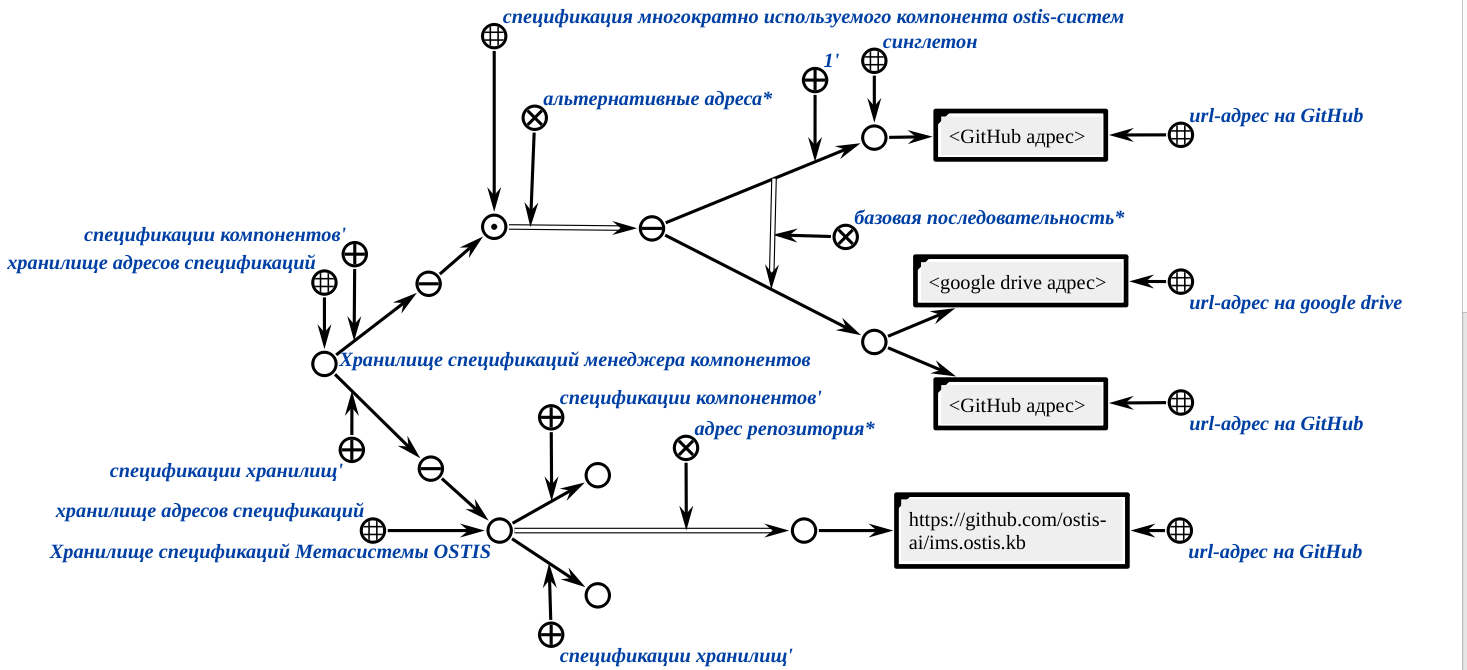
\includegraphics[scale=0.5]{author/part5/figures/specification_storage_addresses.png}
	\label{fig:specification_storage_addresses}
\end{figure}

Если указать адрес корня дерева хранилищ адресов спецификаций, то менеджер компонентов получает доступ ко всем спецификациям дочерних хранилищ. При обработке такого дерева спецификаций менеджер компонентов погружает в sc-память спецификации компонентов, доступных для установки, однако не сами эти компоненты.

\textit{менеджер многократно используемых компонентов ostis-систем} является \myuline{необязательной} подсистемой \textit{ostis-платформы}. Однако система, имеющая менеджер компонентов, может устанавливать компоненты не только сама в себя, но и в другие системы при наличии доступа. Таким образом, одна система может заменить \textit{ostis-платформу} другой системы, оставив при этом \textit{sc-модель кибернетической системы} (см. \textit{\ref{sec_interpreter_ostis_impl}~\nameref{sec_interpreter_ostis_impl}}). Таким же образом некоторая ostis-система может порождать другие ostis-системы, используя компонентный подход.

Включение компонента в \textit{дочернюю ostis-систему} в общем случае состоит из следующих этапов:
\begin{textitemize}
	\item поиск подходящего компонента во множестве доступных библиотек;
	\item выделение компонента в виде, удобном для транспортировки в дочернюю ostis-систему с указанием версии и модификации при необходимости (например, выбор доступного хранилища компонента, выбор оптимального варианта реализации компонента с учетом состава дочерней системы);
	\item установка многократно используемого компонента и его зависимостей (с указанием версии и модификации при необходимости);
	\item интеграция компонента в дочернюю систему;
	\item поиск и устранение ошибок и противоречий в дочерней системе.
\end{textitemize}

Данный процесс с точки зрения пользователя не зависит от типа компонента и особенностей его реализации.

\section*{Заключение Главы \ref{chapter_library}}
\label{ostis_library_conclusion}

Компонентный подход является ключевым в технологии проектирования интеллектуальных компьютерных систем. Вместе с этим, технология компонентного проектирования тесно связана с остальными составляющими \textit{технологии проектирования интеллектуальных компьютерных систем} и обеспечивает их совместимость, производя мощнейший синергетический эффект при использовании всего комплекса частных технологий проектирования интеллектуальных систем. Важнейшим принципом в реализации компонентного подхода является семантическая совместимость многократно используемых компонентов, что позволяет минимизировать участие программистов в создании новых компьютерных систем и в совершенствовании существующих.

Для реализации компонентного подхода в работе предложена \textit{библиотека многократно используемых совместимых компонентов интеллектуальных компьютерных систем на основе Технологии OSTIS}, введена классификация и спецификация многократно используемых компонентов ostis-систем, предложена модель менеджера компонентов, позволяющего взаимодействовать \textit{ostis-системам} с \textit{библиотеками многократно используемых компонентов} и управлять компонентами в системе, рассмотрена архитектура экосистемы \textit{интеллектуальных компьютерных систем} с точки зрения использования библиотеки многократно используемых компонентов.

Полученные результаты позволят повысить эффективность проектирования интеллектуальных систем и средств автоматизации разработки таких систем, а также обеспечить возможность не только разработчику, но и интеллектуальной системе автоматически дополнять систему новыми знаниями и навыками.

%%%%%%%%%%%%%%%%%%%%%%%%% referenc.tex %%%%%%%%%%%%%%%%%%%%%%%%%%%%%%
% sample references
% %
% Use this file as a template for your own input.
%
%%%%%%%%%%%%%%%%%%%%%%%% Springer-Verlag %%%%%%%%%%%%%%%%%%%%%%%%%%
%
% BibTeX users please use
% \bibliographystyle{}
% \bibliography{}
%
\biblstarthook{In view of the parallel print and (chapter-wise) online publication of your book at \url{www.springerlink.com} it has been decided that -- as a genreral rule --  references should be sorted chapter-wise and placed at the end of the individual chapters. However, upon agreement with your contact at Springer you may list your references in a single seperate chapter at the end of your book. Deactivate the class option \texttt{sectrefs} and the \texttt{thebibliography} environment will be put out as a chapter of its own.\\\indent
References may be \textit{cited} in the text either by number (preferred) or by author/year.\footnote{Make sure that all references from the list are cited in the text. Those not cited should be moved to a separate \textit{Further Reading} section or chapter.} If the citatiion in the text is numbered, the reference list should be arranged in ascending order. If the citation in the text is author/year, the reference list should be \textit{sorted} alphabetically and if there are several works by the same author, the following order should be used:
\begin{enumerate}
\item all works by the author alone, ordered chronologically by year of publication
\item all works by the author with a coauthor, ordered alphabetically by coauthor
\item all works by the author with several coauthors, ordered chronologically by year of publication.
\end{enumerate}
The \textit{styling} of references\footnote{Always use the standard abbreviation of a journal's name according to the ISSN \textit{List of Title Word Abbreviations}, see \url{http://www.issn.org/en/node/344}} depends on the subject of your book:
\begin{itemize}
\item The \textit{two} recommended styles for references in books on \textit{mathematical, physical, statistical and computer sciences} are depicted in ~\cite{science-contrib, science-online, science-mono, science-journal, science-DOI} and ~\cite{phys-online, phys-mono, phys-journal, phys-DOI, phys-contrib}.
\item Examples of the most commonly used reference style in books on \textit{Psychology, Social Sciences} are~\cite{psysoc-mono, psysoc-online,psysoc-journal, psysoc-contrib, psysoc-DOI}.
\item Examples for references in books on \textit{Humanities, Linguistics, Philosophy} are~\cite{humlinphil-journal, humlinphil-contrib, humlinphil-mono, humlinphil-online, humlinphil-DOI}.
\item Examples of the basic Springer style used in publications on a wide range of subjects such as \textit{Computer Science, Economics, Engineering, Geosciences, Life Sciences, Medicine, Biomedicine} are ~\cite{basic-contrib, basic-online, basic-journal, basic-DOI, basic-mono}. 
\end{itemize}
}

\begin{thebibliography}{99.}%
% and use \bibitem to create references.
%
% Use the following syntax and markup for your references if 
% the subject of your book is from the field 
% "Mathematics, Physics, Statistics, Computer Science"
%
% Contribution 
\bibitem{science-contrib} Broy, M.: Software engineering --- from auxiliary to key technologies. In: Broy, M., Dener, E. (eds.) Software Pioneers, pp. 10-13. Springer, Heidelberg (2002)
%
% Online Document
\bibitem{science-online} Dod, J.: Effective substances. In: The Dictionary of Substances and Their Effects. Royal Society of Chemistry (1999) Available via DIALOG. \\
\url{http://www.rsc.org/dose/title of subordinate document. Cited 15 Jan 1999}
%
% Monograph
\bibitem{science-mono} Geddes, K.O., Czapor, S.R., Labahn, G.: Algorithms for Computer Algebra. Kluwer, Boston (1992) 
%
% Journal article
\bibitem{science-journal} Hamburger, C.: Quasimonotonicity, regularity and duality for nonlinear systems of partial differential equations. Ann. Mat. Pura. Appl. \textbf{169}, 321--354 (1995)
%
% Journal article by DOI
\bibitem{science-DOI} Slifka, M.K., Whitton, J.L.: Clinical implications of dysregulated cytokine production. J. Mol. Med. (2000) doi: 10.1007/s001090000086 
%
\bigskip

% Use the following (APS) syntax and markup for your references if 
% the subject of your book is from the field 
% "Mathematics, Physics, Statistics, Computer Science"
%
% Online Document
\bibitem{phys-online} J. Dod, in \textit{The Dictionary of Substances and Their Effects}, Royal Society of Chemistry. (Available via DIALOG, 1999), 
\url{http://www.rsc.org/dose/title of subordinate document. Cited 15 Jan 1999}
%
% Monograph
\bibitem{phys-mono} H. Ibach, H. L\"uth, \textit{Solid-State Physics}, 2nd edn. (Springer, New York, 1996), pp. 45-56 
%
% Journal article
\bibitem{phys-journal} S. Preuss, A. Demchuk Jr., M. Stuke, Appl. Phys. A \textbf{61}
%
% Journal article by DOI
\bibitem{phys-DOI} M.K. Slifka, J.L. Whitton, J. Mol. Med., doi: 10.1007/s001090000086
%
% Contribution 
\bibitem{phys-contrib} S.E. Smith, in \textit{Neuromuscular Junction}, ed. by E. Zaimis. Handbook of Experimental Pharmacology, vol 42 (Springer, Heidelberg, 1976), p. 593
%
\bigskip
%
% Use the following syntax and markup for your references if 
% the subject of your book is from the field 
% "Psychology, Social Sciences"
%
%
% Monograph
\bibitem{psysoc-mono} Calfee, R.~C., \& Valencia, R.~R. (1991). \textit{APA guide to preparing manuscripts for journal publication.} Washington, DC: American Psychological Association.
%
% Online Document
\bibitem{psysoc-online} Dod, J. (1999). Effective substances. In: The dictionary of substances and their effects. Royal Society of Chemistry. Available via DIALOG. \\
\url{http://www.rsc.org/dose/Effective substances.} Cited 15 Jan 1999.
%
% Journal article
\bibitem{psysoc-journal} Harris, M., Karper, E., Stacks, G., Hoffman, D., DeNiro, R., Cruz, P., et al. (2001). Writing labs and the Hollywood connection. \textit{J Film} Writing, 44(3), 213--245.
%
% Contribution 
\bibitem{psysoc-contrib} O'Neil, J.~M., \& Egan, J. (1992). Men's and women's gender role journeys: Metaphor for healing, transition, and transformation. In B.~R. Wainrig (Ed.), \textit{Gender issues across the life cycle} (pp. 107--123). New York: Springer.
%
% Journal article by DOI
\bibitem{psysoc-DOI}Kreger, M., Brindis, C.D., Manuel, D.M., Sassoubre, L. (2007). Lessons learned in systems change initiatives: benchmarks and indicators. \textit{American Journal of Community Psychology}, doi: 10.1007/s10464-007-9108-14.
%
%
% Use the following syntax and markup for your references if 
% the subject of your book is from the field 
% "Humanities, Linguistics, Philosophy"
%
\bigskip
%
% Journal article
\bibitem{humlinphil-journal} Alber John, Daniel C. O'Connell, and Sabine Kowal. 2002. Personal perspective in TV interviews. \textit{Pragmatics} 12:257--271
%
% Contribution 
\bibitem{humlinphil-contrib} Cameron, Deborah. 1997. Theoretical debates in feminist linguistics: Questions of sex and gender. In \textit{Gender and discourse}, ed. Ruth Wodak, 99--119. London: Sage Publications.
%
% Monograph
\bibitem{humlinphil-mono} Cameron, Deborah. 1985. \textit{Feminism and linguistic theory.} New York: St. Martin's Press.
%
% Online Document
\bibitem{humlinphil-online} Dod, Jake. 1999. Effective substances. In: The dictionary of substances and their effects. Royal Society of Chemistry. Available via DIALOG. \\
http://www.rsc.org/dose/title of subordinate document. Cited 15 Jan 1999
%
% Journal article by DOI
\bibitem{humlinphil-DOI} Suleiman, Camelia, Daniel C. O'Connell, and Sabine Kowal. 2002. `If you and I, if we, in this later day, lose that sacred fire...': Perspective in political interviews. \textit{Journal of Psycholinguistic Research}. doi: 10.1023/A:1015592129296.
%
%
%
\bigskip
%
%
% Use the following syntax and markup for your references if 
% the subject of your book is from the field 
% "Computer Science, Economics, Engineering, Geosciences, Life Sciences"
%
%
% Contribution 
\bibitem{basic-contrib} Brown B, Aaron M (2001) The politics of nature. In: Smith J (ed) The rise of modern genomics, 3rd edn. Wiley, New York 
%
% Online Document
\bibitem{basic-online} Dod J (1999) Effective Substances. In: The dictionary of substances and their effects. Royal Society of Chemistry. Available via DIALOG. \\
\url{http://www.rsc.org/dose/title of subordinate document. Cited 15 Jan 1999}
%
% Journal article by DOI
\bibitem{basic-DOI} Slifka MK, Whitton JL (2000) Clinical implications of dysregulated cytokine production. J Mol Med, doi: 10.1007/s001090000086
%
% Journal article
\bibitem{basic-journal} Smith J, Jones M Jr, Houghton L et al (1999) Future of health insurance. N Engl J Med 965:325--329
%
% Monograph
\bibitem{basic-mono} South J, Blass B (2001) The future of modern genomics. Blackwell, London 
%
\end{thebibliography}
